\documentclass[a4paper,12pt]{article}
\usepackage[utf8]{inputenc}
\usepackage[english,russian]{babel}
\usepackage{cmap} % correct output encoding

%\usepackage[T2A]{fontenc}
%\usepackage{tempora} 
\usepackage{mathptmx} % russian times new roman

\usepackage[none]{hyphenat} % no word breaks
\sloppy

\usepackage{setspace}
\onehalfspacing

\usepackage{hyperref}
\hypersetup{
	colorlinks=true,
	linkcolor=black,
	citecolor=black,
	urlcolor=cyan
}

\usepackage{graphicx}
\usepackage{pgf}
\graphicspath{{pics/}}
\DeclareGraphicsExtensions{
	.pdf,
	.pgf,
	.png
}

\usepackage{longtable} % split long tables into pages
\usepackage{afterpage}
\usepackage{pdflscape} % turn selected pages
\usepackage{booktabs} % cooler tables
\usepackage{multirow}
\usepackage{amsmath} % unnumbered equations
\usepackage{tabularx}

\usepackage{geometry}
\geometry{
	top=20mm,
	bottom=20mm,
	left=25mm,
	right=20mm
}

\usepackage[
	style=apa,
	doi=false,
	backend=biber, 
	natbib
]{biblatex}
\addbibresource{ref.bib}

\usepackage{comment} % comment

\let\oldsection\section
\renewcommand\section{\clearpage\oldsection}

\begin{document}

\begin{center}
	Федеральное государственное автономное образовательное учреждение высшего образования «Национальный исследовательский университет «Высшая школа экономики»
	\\
	\bigskip
	Санкт-Петербургская Школа экономики и менеджмента \\
	Образовательная Программа "Экономика"
\end{center}

\vspace{8em}

\begin{center}
	{\Large КУРСОВАЯ РАБОТА}\\
	\textsc{\textbf{
			На тему
			\linebreak
			"Применение гравитационной модели к анализу миграций в Российской империи"}}
\end{center}

\vspace{2em}

\hfill\parbox{16cm}{
	\hspace*{5cm}\hspace*{-5cm}Выполнил студент группы БЭК-182\\
	Соснин Юрий Алексеевич\\
	
	\hspace*{5cm}\hspace*{-5cm}Научный руководитель:\\
	ст.преп. Куга Яков Тойвович\\
}

\vspace{\fill}

\begin{center}
	Санкт-Петербург
	
	2021 г.
\end{center}
\thispagestyle{empty}

\clearpage


\tableofcontents


\section{Введение}

\begin{comment}
Внутренняя миграция - один из важных вопросов экономики развития. Миграция перераспределяет рабочую силу в пространстве, уравновешивая рынки и производя более эффективные экономические результаты. Для развивающихся стран внутренняя миграция имеет еще большее значение: это, в первую очередь, урбанизация, переселение сельскохозяйственных работников в города, где они становятся рабочими и удовлетворяют растущие потребности индустриальной экономики.

Хотя внутренняя миграция в развитых в современных развивиющихся странах изучена подробно, мы мало знаем о внутренней миграции в индустриализующихся странах - например, Российской империи второй половины 19 века.

The size and intensity of migration flows depend on circumstances in the place of origin,
which could be push factors, and those in the destination, which could be pull factors. Migrants subjectively evaluate economic, psychological, and social reasons for moving (Todaro 1980).
Faggian et al. (2015) review regional science contributions on interregional migration determinants. One of the key aspects is migration’s role as automatic stabilizer of utility over space.


у развития и мигарции интересные взаимоотношения. сала-и-мартин, т.д.
фундаментальные причины миграции -- то и то.
гравитацоинная модель.

я про РИ.
recent studies (markevich) показывают развитие. я исследую миграции. 
\Маркевич отмечает развитие. Я отмечу миграции.\

с помощью данный я отвечаю на исследовательский впрос.

structured as follows.


Стоит сказать, что связь миграции и экономического развития породила несколько важных проблем и направлений экономической науки. Во-первых, это migration-development nexus, правда, в основном для интернациональных миграций (см., например, \cite{migration_development_2010, letouze_nexus_2009}). Другая проблема -- это региональная сходимость, regional convergence, и вопрос о том, проводят ли внутренние миграции к выравниванию экономических характеристик регионов (см. \cite{barro_convergence_1992} и, например, \cite{reichlin_diverging_1998}). Обе эти важные проблемы находятся, тем не менее, за пределами данной работы. То, что интересует меня -- это обратная зависимость -- действительно ли мигранты едут в более развитые регионы, и регионы с большим населением.


Furthermore, there has been much debate in the literature on the linkage between
migration and development. But, it is straightforward to conclude that development and
internal migration are complements. A growing body of empirical studies claims that
development fuels and stimulates migration rather than reduces it, at least in the short and
medium run (Lucas 2014), while others consider migration as an important vehicle for
boosting development in both origin and destination location (Phan and Coxhead 2010).
The development-migration relationship remains the focus of attention of a large body of
research investigating several empirical questions with normative and policy implications
(Bell et al. 2015).
\end{comment}

Связь экономического развития и миграции -- большой и сложный вопрос современной экономики развития.
% что-то! тут необходимо вкинуть пару ссылок
Тем не менее, можно с уверенностью сказать, что миграции и экономическое развитие тесно связаны между собой.

Фундаментальные причины миграции -- это разница в полезностях индивидов, принимающих решение о переезде, но на макро-уровне ее можно объяснить с помощью характеристик регионов. 
Некоторые свойства территорий, такие как, например, высокая безработица, выступают <<выталкивающими>>, push-факторами для региона-источника миграции; низкая безработица в регионе-реципиенте, с другой стороны, это pull-фактор, <<притягивающий>> потенциальных мигрантов. Аналогия с гравитацией неслучайна -- наверное, самая популярная модель, применяемая к миграциям населения -- это гравитационная модель, прямая аналогия с законом Ньютона. Оценка гравитационной модели на данных о двухсторонних взаимодействиях позволяет определить причины, стоящие за решениями о миграции и выборе ее направления.

Моя работа посвящена внутренней миграции в Российской империи в конце 19 века. Последние исследования собирают все больше информации об экономике России перед Первой мировой войной \citep{markevich_abolition_2018, cheremukhin_industrialization_2017} и о региональном распределении экономического развития \citep{markevich_regional_2019, lindert_inequality_2014}.
И хотя исследованию причин внутренней миграции в других великих державах 19 века посвящено некоторое направление литературы о исторической демографии, работы о России очень немногочисленны \citep{anderson_internal_1980, leasure_internal_1968}, и им недостает экономической методологии и современного взгляда.

Я использую данные Всероссийской переписи населения 1897 года \citep{census_1897} о миграции и некоторых других показателях, а также набор других исторических источников, чтобы выяснить, какие региональные факторы оказывали влияние на внутреннюю миграцию в конце 19 века в России. Среди региональных факторов, наиболее часто считающихся детерминантами миграций и индустриальных экономиках -- демографические (плотность населения, уровень урбанизации), экономические (характеристики рынка труда и индустриальный выпуск) и социальные (уровень грамотности). Я проверяю гипотезы относительно этих переменных для миграции в города и уезды империи.
% вопрос такой себе, но вкад есть

\begin{comment}
Оказывалось ли перенаселение региона фактором, вытесняющим мигрантов в другие места? Ехали ли мигранты преимущественно в промышленные городские центры, или наиболее значимым было переселение крестьян в плодородные окраины? В конце концов, были ли детерминанты внутренней миграции сопоставимы в России и Великобритании или Германии, того же периода? На эти вопросы я постараюсь ответить в данной работе.

Интерес к истории империи возрастает в последнее -- стоит отметить работы Маркевича об экономической истории или Б. Миронова о социальной. 
История может помочь ответить на современные вопросы. И хотя данная работа не посвящена какому-нибудь знаменитому ворпосу, я вношу вклад. %куда?
\end{comment}

Работа структурирована следующим образом. Сначала я рассказываю о гравитационной модели и способах ее оценки в секциях 1.1 и 1.2. Далее -- о ее применении к внутренней миграции в современных развивающихся странах и к историческим миграциям в европейских странах в 19 веке. После этого, я кратко рассказываю о Российской империи в 19 веке и задаю исследовательский вопрос. В практической части сначала идет обсуждение данных и их описательные статистики, затем -- я обсуждаю гипотезы и модель, и наконец, результаты. Заканчивается работа заключением, обсуждающим ограничения результатов и дальнейшее обсуждение.

\begin{comment}
Актуальность исследования
Задачи
Объект исследования
Значимость
Степень изученности темы
Новизна
Характеристика базы исследований
Описание структуры работы
\end{comment}

\section{Анализ внутренней миграции}

\subsection{Гравитационная модель}

Впервые основные гипотезы пространственного моделирования миграций предложил в 1885 году британский географ и статистик Эрнст Георг Равенштайн в знаменитой статье \emph{The Laws of Migration} в \emph{Journal of the Royal Statistical Society}. \citep{ravenstein_laws_1885} Автор проанализировал данные британских переписей 1871 и 1881 годов, определяя основные направления и силу потоков внутренней миграции между Англией, Шотландией и Ирландией, а также между графствами внутри этих королевств. Равенштайн не предложил математической модели миграции, его анализ напоминает скорее современную описательную статистику, однако на основе своих наблюдений он сформулировал несколько гипотез -- <<законы миграции>>, легшие в основу будущих моделей.

\begin{comment}
Во-первых, Равенштайн отмечает, что основная причина миграции – рынок труда. Жители Британии чаще переселялись в торговые и промышленные центры, с более широкими возможностями для трудоустройства.

Во-вторых, автор отмечает отрицательную роль расстояния и других пространственных характеристик в силе миграционных потоков. В первую очередь, города привлекают жителей близлежащей сельской местности, потом – жителей соседних графств, и, наконец, жителей остальной страны (морское сообщение, при этом, также способствует миграции). Сама сила миграционного потока также, очевидно, зависит от населения, готового принимать в нем участие.

С другой стороны, даже между самыми дальними регионами есть двустороннее миграционное «сообщение». Каждый поток имеет противоположный.

Наконец, мигранты имеют особые характеристики: молодые, не имеющие детей, и жители деревень более предрасположены к миграции, чем, соответственно, более взрослые, жители города и семьи с детьми. Кроме того, в случае Британии 19 века, женщины более мобильны, чем мужчины. 

Работа Равенштайна оказала значительное влияние на будущие работы демографов, социологов, и, в конечном счете, экономистов, определив основные гипотезы для моделей миграции и пространственного взаимодействия в целом. 
\end{comment}

Во-первых, автор отмечает роль расстояния в миграционных потоках: большинство мигрантов преодолевают небольшое расстояние. Кроме того, <<... we must take into account the number of natives of each county that furnishes the migrants, as also the population of the towns or districts which absorb them>> -- 
сила миграционного потока зависит от населения, готового принимать в нем участие, от способности регионов отдавать и принимать мигрантов.

Во-вторых, миграции имеют определенную пространственную структуру. В первую очередь, города привлекают жителей близлежащей сельской местности, потом – жителей соседних графств, и, наконец, жителей остальной страны (морское сообщение, при этом, также способствует миграции). С другой стороны, даже между самыми дальними регионами есть двустороннее миграционное «сообщение». Каждый поток имеет противоположный.

В-третьих, Равенштайн отмечает, что основная причина миграции – рынок труда. Жители Британии чаще переселялись в торговые и промышленные центры, с более широкими возможностями для трудоустройства.

Наконец, мигранты имеют особые характеристики: молодые, не имеющие детей, и жители деревень более предрасположены к миграции, чем, соответственно, более взрослые, жители города и семьи с детьми. Кроме того, в случае Британии 19 века, женщины более мобильны, чем мужчины. 

Работа Равенштайна оказала значительное влияние на будущие работы демографов, социологов, и, в конечном счете, экономистов, определив основные гипотезы для моделей миграции и пространственного взаимодействия в целом. Первый закон миграции в понимании Равенштайна, например, излагает положения базовой гравитационной модели.

В дальнейшем работа над моделями миграции населения продолжилась. \citeauthor{stouffer_intervening_1940} расширил определение расстояния до <<intervening opportunities>> -- всех препятствующих переезду факторов (транспортные расходы, информация о месте назначения, законодательные барьеры, культурные отличия и так далее) \citep{stouffer_intervening_1940}. Позднее была предложена гравитационная модель -- модель двухстороннего пространственного социального взаимодействия - основанная на Ньютоновском законе гравитации \citep{stewart_demographic_1948, zipf_p1_1946}. Изначально включавшая в себя только населения источника и назначения и расстояние, она была расширена включением push- и pull-факторов -- доходов, климата, качества социальной политики, безработицы, и т.д. \citep{lee_theory_1966}. 
Одновременно с этим развивалась применение модели к международной торговле, где она оказалась также успешной \citep{de_benedictis_gravity_2011}.

\begin{comment}

Американский социолог Самуэль Стоффер в статье «Intervening opportunities: a theory relating mobility and distance» продолжил развивать идею о влиянии расстояния на миграционные потоки. Согласно его теории, не cтолько расстояние имеет значение, сколько так называемые intervening opportunities – транспортные расходы, информация о месте назначения, законодательные барьеры, культурные отличия и так далее. \citep{stouffer_intervening_1940}

Гравитационная модель – модель двухстороннего пространственного социального взаимодействия – впервые была сформулирована John Q. Stewart в 1948 году, как аналогия физическому закону Ньютона. \citep{stewart_demographic_1948} Вся статья пронизана физическими аналогиями: например, отдельные люди сравниваются с молекулами газа, а большие группы людей – с самим газом. На этом основании он критикует получивших распространение к тому времени микро-подход, изучающий отдельных людей и их мотивацию – если бы физики изучали только молекулы, законов, описывающих свойство газов, не существовало бы.

Предложенная Stewart модель выглядела так: 

\begin{equation*}
	F = \frac{G(N_{1\mu_1})(N_{2\mu_2}))}{d^2}
\end{equation*}

Автор привел несколько эмпирических примеров своего «закона», однако не догадался сделать степени при переменных вариативными – для него фиксированные числа, аналогичные физическим константам.

Чуть ранее Стюарта, Зипф в своих работах показал, что коэффициент (степень) расстояния для Соединенных Штатов на самом деле не 2, а ближе к единице, и объяснил это своими социологическими аргументами, а не просто аналогией с физикой. \citep{zipf_p1_1946} Стоит отметить, что Зипф применяет модель уже не только к миграции, но и, в частности, к обмену товарами между городами – сейчас, гравитационная модель даже «популярнее» в применении к международной торговле, чем к миграциям.

\cite{lee_theory_1966} в работе <<A theory of migration>> выдвинул гипотезы о том, что решение о миграции, кроме личных качеств мигранта и intervening obstacles, зависит от характеристик региона – push- и pull-факторов – доходов, климата, качества социальной политики, безработицы, и всех возможных других, различающихся по значению для каждого мигранта.

С этого времени начинается теоретическое и эмпирическое развитие гравитационной модели. Ученые продолжают вносить вклад в теперь уже целый класс special interaction gravity models.

\end{comment}

Современная форма базовой гравитационной модели миграции выглядит так:

\begin{equation}\label{eq:base}
	M_{ij} = \beta_0 P^{\beta_1}_{i} P^{\beta_2}_{j} D^{\beta_3}_{ij} + \varepsilon_{ij}
\end{equation}

Здесь, $M$ – число переселенцев из региона $i$ в регион $j$; $P_i$ и $P_j$ – население региона-источника и региона-назначения, $D_{ij}$ – расстояние, $\varepsilon_{ij}$ - случайный фактор. Расширенная модель кроме населения будет также включать всевозможные притягивающие и отталкивающие характеристики регионов, а расстояние не обязательно должно быть географическим.

Сегодня, гравитационная модель миграции -- уже не просто результат эмпирических наблюдений за миграционными потоками. В отличие от школы <<социальной физики>>, к которой принадлежали первые авторы модели, экономистам необходима связь между эмпирическими макро-законы и решениями индивидов, максимизирующих полезность, микро-основания. 
Основное микроэкономическое объяснение гравитационных моделей с помощью решений индивидов – модель максимизации случайной полезности (Random utility maximization, RUM) (см., например, \cite{beine_practitioners_2016}).
О сновании модель RUM лежит полезность от переезда в другой регион, определенная как разность детерминированной полезности нахождения в том регионе и издержек на переезд, плюс случайный ненаблюдаемый фактор. Предположение о распределении этого фактора определяет ожидаемую вероятность того, что выбор определенного альтернативного региона окажется оптимальным выбором индивида. От этого можно перейти к ожидаемой суммарной миграции между регионами, которая оказывается положительно зависящей от привлекательности региона-реципиента и его способности отдавать мигрантов, и отрицательно -- от привлекательности региона-источника и его <<доступности>>, что соответствует выражению гравитационной модели.

\begin{comment}
Модели RUM описывают полезность, которую человек получает от проживания в регионе, по сравнению с ожидаемой полезностью, которую он может получить при переезде в альтернативные места назначения. Сравнение включает в себя как ожидаемые выгоды (такие как более высокие ожидаемые доходы), так и затраты на миграцию.


The theoretical basis for gravity models of migration is generally represented by a random utility maximization (RUM) model (see [1], [2], and [3], among others). RUM models describe the utility that an individual receives from living in a particular country compared to the expected utility received if moving to alternative destinations. The comparison involves both expected benefits (i.e. factors increasing the attractiveness of the destination such as higher expected earnings) and costs of migrating from origin to destination (such as distance or unfavorable migration policies).

The RUM model also includes a component that captures the unobserved factors of the individual utility associated with each choice. The researchers’ assumptions regarding the statistical uncertainty around this component determine the expected probability that an individual will maximize his/her utility by opting for a particular destination. For instance, a logit-normal distribution can be adopted in such a way that the expected gross migration flows from one country to any other depend on the characteristics of the origin country, the attractiveness of the destination, and the accessibility of the destination country for potential migrants, which are criteria that clearly resemble a gravity model [1]. One relevant assumption of the RUM model is that the attractiveness of a destination is not supposed to be affected by migration. For instance, if one particular destination is attractive due to its low levels of unemployment when compared to a particular origin, massive inflows of immigrants could increase unemployment in the destination while at the same time decreasing it in the origin country. Gravity models do not capture these second-round effects, which is an important point to consider in order to appropriately interpret the model’s results.

In any case, RUM models provide an appropriate theoretical justification of the intuition behind gravity models. The use of RUM models makes clear what the assumptions made by researchers are, and how these assumptions yield different specifications of empirical gravity models.

1 = Grogger, J., and G. H. Hanson. “Income maximization and the selection and sorting of
international migrants.” Journal of Development Economics 95:1 (2011): 42–57.
2 = Ortega, F., and G. Peri. “The effect of income and immigration policies on international
migration.” Migration Studies 1:1 (2013): 47–74.
3 = Beine, M., and C. Parsons. “Climatic factors as determinants of international migration.”
Scandinavian Journal of Economics 117:2 (2015): 723–767
\end{comment}

% \subsection{Методы оценки}\label{sec:ppml}

Есть несколько методов оценки гравитационной модели, самым очевидным из которых является МНК с логарифмическим преобразованием.

\begin{equation}\label{eq:log}
	ln(M_{ij}) = \beta_0 + {\beta_1}ln(P_{i}) + {\beta_2}ln(P_{j}) + {\beta_3}ln(D_{ij}) + \varepsilon_{ij}
\end{equation}

Несмотря на удобство и простоту интерпретации, такая спецификация имеет ряд недостатков \citep{silva_log_2006}. Во-первых, логарифм от нуля не определен, тогда как нулевые миграционные потоки часто составляют заметную часть наблюдений. Два основных способа решения этой проблемы – это исключение нулевых наблюдений и прибавление к M небольшой константы, как правило 1 или 0,5. При этом исключение наблюдений с нулями смещает оценку, но и размер константы невозможно определить теоретически, что снижает точность и обоснованность оценок логарифмической модели. 

Если и другая, теоретическая проблема с логарифмированием моделей с постоянной эластичностью, или мультипликативных моделей, отмеченная \citeauthor{silva_log_2006}. Чтобы случайный фактор в логарифмической спецификации не зависел от регрессоров, нужно сделать насчет него очень строгие предположения, что в большинстве случаев нереалистично -- поэтому \citeauthor{silva_log_2006} не рекомендуют логарифмировать гравитационные модели. 

Вместо этого, авторы предложили использовать метод Poisson pseudo-maximum-likelihood. Этот метод естественным образом справляется с нулями в данных, оценивая модель в ее мультипликативной форме с помощью метода максимального правдоподобия. Предполагается, что миграционные потоки распределены по Пуассону с условным средним $\mu_{ij}$, которое является функцией объясняющих переменных. Формально это определяется следующим образом:

\begin{gather*}\label{eq:poisson0}
	Pr[M_{ij}] = \frac{exp(-\mu_{ij})\mu^{M_{ij}}_{ij}}{M_{ij}!},\quad M_{ij} = (0, 1, ...) \\
	\mu_{ij} = exp(\beta_0 + P_i \beta_1^T + P_{j} \beta_2^T + D_{ij} \beta_3^T)
\end{gather*}

% очень важно сделать это правильно и адекватно, представь что это читает Пырлик - он не должен испытывать кринж!
% мб тут про фиксед эффекты поговорить? что есть и другие методы

Такая оценка стала в последнее время бенчмарком в исследованиях с применением гравитационной модели, все больше авторов предпочитают ее логарифмам.

В целом, спецификации гравитационной модели выходит далеко за рамки расширенной гравитационной модели. Использование панельных данных позволяет применить фиксированные эффекты для источника, реципиента и для пар регионов; random intercept позволяет при этом оценить и неизменные факторы регионов. Тем не менее, моя работа -- в силу доступности данных -- кросс-секционная, и применять я буду PPML estimator для расширенной модели.

% ну что это за кринж, мб лучше убрать?

\subsection{Миграция в развивающихся странах}

Итак, гравитационные модели активно и успешно применяются к анализу внутренней миграции в современных странах \citep{andrienko_determinants_2004, guriev_breaking_2015, molloy_internal_2011, etzo_internal_2008}.
Основной фокус обзора литературы, однако, будет направлен на литературу о миграциях в 19 веке -- но прежде чем перейти к таким работам (которые, по большей части, написаны в 80-х годах прошлого века), стоит все-же обратиться к современным применениям гравитационных моделей миграции. Будут рассмотрены примеры статей, посвященных современным развивающимся странам. 
Предположение о том, что современных развивающиеся страны похожи на страны Европы в период индустриализации, конечно, далеко от того, чтобы быть истинным в полной мере, однако многие процессы можно назвать схожими -- в частности, урбанизация, развитие промышленности и концентрация населения -- происходили в Европе 18-19 веков, происходят и в развивающихся странах в недавнем прошлом. 
Я не буду в этом обзоре обращать внимание на все, или даже на самые популярные; основная цель – составить представление о том, какие гипотезы проверяют авторы и какие переменные в целом используют.

В большинстве работ о внутренней миграции с применением гравитационной модели авторы стремятся, оценив расширенную гравитационную модель, определить региональные детерминанты миграции. В работах обсуждается, какие характеристики регионов в целом оказывают влияние на перемещение населения, а также проверяются гипотезы относительно конкретных переменных. В качестве данных используют панели, основанные на переписях населения; оценивают гравитационные модели либо обычным МНК, либо с помощью PPML -- эта техника становится все популярнее в последние годы.

Несколько примеров работ, посвященных миграции в развивающихся странах. Так, \citeauthor{mexico_2013} проверяют влияние на миграции либерализации внешней торговли в результате вступления Мексики в НАФТА \citep{mexico_2013}.
\citeauthor{tunis_2018} выясняет, как на внутренние миграции в Тунисе влияют безработица, количество доступных вакансий и расходы домохозяйств \citep{tunis_2018}.
\citeauthor{vietnam_1997} обнаруживают, что мигранты стремятся в более индустриализованные и богатые регионы, а государственные программы, призванные этому помешать почти не оказывают никакого влияния \citep{vietnam_1997}; \citeauthor{indonesia_2012} приходит к таким же выводам для Индонезии \citep{indonesia_2012}.
\citeauthor{vietnam_2020} находит положительную связь между внутренними миграциями и качеством государственного управления во Вьетнаме \citep{vietnam_2020}.
\citeauthor{india_2018} определяют, что границы штатов в Индии негативно влияют на миграцию в масштабе районов -- правда, авторы контролируют только на национальные различия, но не на экономические факторы \citep{india_2018}.

\citeauthor{indonesia_2017} и \citeauthor{equador_2018} используют гравитационные модели для подтверждения гипотезы о концентрации населения. И в Эквадоре, и в Индонезии, развивающихся странах, миграции направлены в крупные города, то есть регионы с высоким уровнем урбанизации и высоким населением. 
Население, таким образом, концентрируется в нескольких агломерациях, города и регионы с уже высоким населением продолжают расти, притягивая жителей менее населенных районов сильнее, чем это происходит в обратном направлении. 
В обоих случаях, тем не менее, этот тренд ослабевает с течением времени.

% Вообще, экономические и социальные характеристики регионов являются главными, помимо населения и расстояния, переменными в гравитационных моделях для развивающихся стран. Почти во всех работах, так или иначе, в качестве предикторов выступают плотность населения, уровень урбанизации, доходы и структура занятости. Как правило, миграции оказываются направлены из менее развитых регионов в более развитые -- мигрантов <<притягивают>> возможности трудоустройства в более урбанизированных и промышленно развитых областях, что полностью соотносится с микроэкономическими обоснованиями гравитационных моделей.

\citet{etzo_internal_2008} выделяет 4 основные группы переменных расширенной гравитационной модели:
\begin{enumerate}
	\item Гравитационные переменные
	\item Экономические переменные
	\item Переменные рынка труда
	\item Переменные <<окружающей среды>>
\end{enumerate}

Рассмотренные статьи подтверждают такие приоритеты. Экономические и социально-экономические характеристики регионов являются главными, помимо населения и расстояния, переменными в моделях для развивающихся стран. Во многих работах, так или иначе, в качестве предикторов выступают плотность населения, уровень урбанизации, структура занятости или уровень безработицы. Немногие, правда, применяют географические контроли -- отчасти потому, что рассмотренные страны, как правило, являются довольно однородными в этом плане, чего нельзя будет сказать о России.

Во всех рассмотренных работах, миграции оказываются направлены из менее развитых регионов в более развитые -- мигрантов <<притягивают>> возможности трудоустройства в более урбанизированных и промышленно развитых областях, что полностью соотносится с микроэкономическими обоснованиями гравитационных моделей.

\begin{comment}
Стоит сказать, что связь миграции и экономического развития породила несколько важных проблем и направлений экономической науки. Во-первых, это migration-development nexus, правда, в основном для интернациональных миграций (см., например, \cite{migration_development_2010, letouze_nexus_2009}). Другая проблема -- это региональная сходимость, regional convergence, и вопрос о том, проводят ли внутренние миграции к выравниванию экономических характеристик регионов (см. \cite{barro_convergence_1992} и, например, \cite{reichlin_diverging_1998}). Обе эти важные проблемы находятся, тем не менее, за пределами данной работы. То, что интересует меня -- это обратная зависимость -- действительно ли мигранты едут в более развитые регионы, и регионы с большим населением.
\end{comment}

\begin{comment}
%На второй вопрос пытаются авторы другой категории статей.
%\citeauthor{indonesia_2017} проверяют теорию \citeauthor{long_migration_1985} на данных миграций в Индонезии.
% Другой класс работ связывает внутреннюю миграцию с концентрацией населения. 
%Согласно модели \citeauthor{long_migration_1985}, функция концентрации населения относительно степени экономического развития общества <<выпукла вверх>>. \citep{long_migration_1985} 
%В начале процесса индустриализации урбанизация и высокая плотность населения эффективны: они позволяют поддерживать эффект масштаба. Так как мигранты переезжают из слаборазвитых сельских районов в развитые городские центры (что уже обсуждалось), %в поисках более высокой заработной платы, лучших возможностей трудоустройства в целом и лучших условий труда, возможностей получения образования. 
%города и регионы с уже высоким населением продолжают расти, притягивая жителей менее населенных районов сильнее, чем это происходит в обратном направлении. 
%По мере развития технологий транспорта и обмена информацией, однако, происходит обратный процесс субурбанизации и деурбанизации, снижающие издержки <<тесноты>> (congestion) -- население перераспределяется более равномерно в географическом смысле. 
%В контексте статьи, это означает, что % что?


% Эту гипотезу проверяют для Индонезии \citep{equador_2018, indonesia_2017}. 
% Какой-то пересказ Индонезии

%Другая работа, посвященная перераспределению населения % -- Эквадор
%В обоих случаях, значительной оказывается концентрация населения в крупнейших столичных регионах стран. 
\end{comment}

% Какие переменные, как оценивают? Какие гипотезы?
% Выводы для всех: едут в более хорошие, по меркам гдп и рынка труда
% Для истории это так же! → и в следующую главу – ой как круто!
% Соответственно, переписать все чтобы было логично!
% Прежде чем писать результаты, надо на 100/% переписать все остальное и Россию тоже – хотя бы каркас и вторую часть про статью Маркевича и исследовательский вопрос.

\subsection{Внутренние миграции в 19 веке}

% Работы, посвященные экономической истории, миграциям в 19 веке, немногочисленны и по большей части устаревши, несмотря на то что статистические данные в странах Европы для этого времени уже доступны в достаточном количестве и качестве. Большое внимание уделено Великобритании.

Интересно заметить, что статья Равенштайна \citeyear{ravenstein_laws_1885}, положившая начало пространственным количественным исследованиям внутренней миграции, сегодня может считаться и исторической: объект работы -- Британия 19 века, миграции исследуются в контексте эпохи индустриальной экономики до Первой мировой войны, источник -- данные переписей. 

Позднее, исследователи снова обратили внимание на европейскую историю: существует направление исторической демографии, занимающееся анализом внутренней миграции в странах Европы для этого времени. 
Тем не менее, сейчас эти работы по большей части устаревши. Кроме того, несмотря на доступность исторических данных, таких работ немного:
\citeauthor{mcquillan_economic_1980} в \emph{Economic Factors and Internal Migration: The Case of Nineteenth-Century England} (\citeyear{mcquillan_economic_1980}), описывая состояние литературы по проблеме внутренней миграции в историческом контексте, отмечает, что ей уделено мало внимания. Это было справедливо в 80-х годах прошлого века, отчасти справедливо и по сей день.
Все работы -- это либо демографические работы, описывающие основные направления и особенности миграционных потоков, либо исторические case-study, описывающие особенности миграции небольших групп; немного внимания уделено экономическим исследованиям причин межрегиональной миграций в масштабе стран. 

Сам \citeauthor{mcquillan_economic_1980} не применяет тогда уже разработанную гравитационную модель – для определения детерминант миграции он рассматривает корреляции между темпом out-migration и объясняющими переменными, такими, как доля занятых в сельском хозяйстве, доля нищих, доход и географическая площадь. Данные, используемые в исследовании – переписи населения в Англии 1851-1901 годов. Методология таких работ, конечно, вызывает вопросы. Современные методы (в т.ч. гравитационные модели) позволяют ответить на вопросы о макро-причинах миграции с большей достоверностью.

\citet{greenwood_geographic_1973} применяют гравитационную модель с сельскохозяйственными доходами к миграциям в Англии и Уэльсе в 19 веке. Авторы приходят к выводу, что внутренняя миграция отрицательно зависела от сельскохозяйственных доходов в регионе-источнике, положительно – от возможностей индустриального трудоустройства в регионе-направления, и стандартно негативно – от расстояния. В противоположность гипотезе Равенштайна, миграция на большое расстояние не оправдывалась индустриальным развитием: в целом, города привлекали трудовые ресурсы из близлежащих регионов с низкими сельскохозяйственными доходами.

Другая статья о миграции в Великобритании, \emph{Internal migration in England, 1818-1839}, фокусируясь на другом периоде, периоде более ранней индустриализации, отвечает на похожие вопросы \citep{nicholas_internal_1987}. Используя данные о сосланных в Австралию жителей Англии (которые оказываются относительно репрезентативны относительно всего населения Англии), исследователи заключают, что различия в степени урбанизации, как прокси для возможностей трудоустройства, негативно влияли на поток миграции между регионами; уровень грамотности, как в регионе-источнике, так и в регионе-реципиенте, имел положительный знак; сельскохозяйственные доходы показывали такие же зависимости, как и для более поздних периодов.

% вот эти 3 запихать в один абзац про вб

Использование необычных микро-данных для гравитационной модели нередко помогает исследователям в более ранние периоды истории. \citeauthor{charpentier_internal_2018}, например, используют данные генеалогических деревьев с сайта Geneanet, чтобы отследить миграции во Франции в начале 19 века. В целом, исследования миграции в период до индустриализации или ранней индустриализации в Европе составляют значительную часть литературы. Кроме Англии и Франции, \citeauthor{mccants_internal_1992} анализирует внутреннюю миграцию во Фрисландии, историческом регионе на севере Нидерландов в период 1750-1805 годов \citep{mccants_internal_1992}.  Автор, правда, не использует расширенную гравитационную модель, зато доказывает, что представление о резком увеличении темпов внутренней миграцией неверно: население Европы было довольно мобильно и в более ранние периоды, особенно на короткие расстояния.

Как можно заметить, основное внимание в литературе, в продолжение традиции Равенштайна, уделено Великобритании. При этом стоит отметить также работы, посвященные Германии, Испании и Италии в конце 19 – начале 20 века \citep{silvestre_internal_2005, hochstadt_migration_1981, hogan_migration_1985}.

Исследования внутренней миграции в Европе 19 века не сильно отличаются от работ о современных развивающихся странах. Проверяются те же гипотезы: мигранты предпочитают перемещаться в более богатые, промышленно развитые и урбанизированные регионы, что в 19 веке, что сейчас.

% Какой-то переход к России?

Что касается России, есть всего несколько работ, посвященных количественному исследованию внутренних миграций в Российской империи конца 19 – начала 20 века. Статья \citeauthor{leasure_internal_1968} и монография Барбары Андерсон \citep{anderson_internal_1980} наиболее близки к теме данной работы: они анализируют межрегиональные миграции по данным переписи 1897 года с помощью макро-моделей и пытаются выявить характеристики регионов, влиявшие на миграционные потоки.

Leisure и Lewis в 1968 году предприняли попытку, используя данный переписи, определить, были ли мигранты в Российской империи более склонны переезжать в более развитые регионы с большими доходами. \citep{leasure_internal_1968} Оказалось, что степень урбанизации, уровень грамотности и процент занятых в промышленности связан с более высокими уровнями миграции в регион, а занятость в сельском хозяйстве – с более низким уровнем.

% Но у меня же не так?

Исследовательский вопрос и результаты схожи с вопросами и результатами в литературе, касающейся других стран, однако методы по современным меркам оставляют желать лучшего. В частности, авторы не используют гравитационную модель, наиболее подходящую для такого рода исследования, но, более того, даже не рассматривают все имеющиеся данные. <<Because it was much too laborious to calculate and analyze in-migration to each guberniia from each of the other eighty-eight guberniias or foreign countries ..., it was decided to consider for each guberniia only the top five suppliers of migrants>>. Кроме того, как метод определения зависимости авторы использовали ранговую корреляцию Пирсона, вместо регрессий, а также не включили достаточного количества переменных контроля. Несмотря на недостатки, эта статья -- по-прежнему одна из немногих, посвященных вопросу миграции в Российской империи.

Барбара Андерсон в монографии 1980 года выдвигает нетипичную гипотезу: выбор направления миграции зависит не столько от экономических показателей, сколько от <<схожести>> места назначения с изначальным местом жительства мигранта. Даже неграмотный потенциальный мигрант из региона с высоким уровнем грамотности будет иметь более <<современные>> взгляды на жизнь и будет предпочитать переезд в регион с высоким уровнем грамотности; то же самое и с естественным приростом населения и промышленным выпуском. Автор тоже не применяет гравитационную модель, вместо этого оценивая регрессии для миграции в отдельные регионы из других регионов, с расстоянием, грамотностью, естественным приростом населения, выпуском промышленности и производительностью земли в качестве зависимых переменных. Б. Андерсон делит страну на несколько больших регионов в зависимости от их <<modernity>>, и анализирует миграции внутри них. В целом, гипотезы подтверждаются: более современные регионы привлекали мигрантов из более современных регионов в смысле уровня грамотности, структуры трудоустройства и прироста населения (он рассматривается как мера стадии демографического перехода и сам по себе оказывается притягивающим фактором, что противоречит результатам для других стран).
Тем не менее, малое количество использованных данных (по 20-50 наблюдений в одной регрессии), недостаточное количество переменных контроля (культурные различия между регионами или географические характеристики регионов не используются) ставят под сомнение результаты исследования.

% И славик и барбара приходят в выводу о том, что мигранты в Российской империи предпочитали переезжать в более развитые регионы ?
% Отмечают два основных направления миграции: в крупные города и на земли фронтира.
% Куда-то это надо написать

И \citeauthor{leasure_internal_1968}, и \citeauthor{anderson_internal_1980} отмечают наличие других данных о миграции в поздней Российской империи – это данные о переселении крестьян в Сибирь и на Дальний восток незадолго до и во время реформ Столыпина \citep{itogi_1910, itogi_1916}. Они не в полной мере подходили для двух предыдущих работ, не будут использоваться и в данной курсовой, однако на них основана самая заметная работа о внутренней миграции в РИ -- статья А. Маркевича и др. \emph{Property rights and internal migration}.

\citeauthor{chernina_property_2014} исследуют связь внутренней миграции и ликвидности земли. Реформа Столыпина, кроме прочего, позволила крестьянам некоторых центральных губерний выходить из передельных общин, получая право собственности на свою землю, и, соответственно, возможность ее продать. Рассматривая реформу как естественный эксперимент, повлиявший на провинции с передельными общинами и не повлиявший на другие губернии и области, авторы, с помощью панельных данных о переселении крестьян за Урал в 1901-1914, показывают, что изменение прав собственности на землю увеличило миграцию независимо от других аспектов реформы.

% Какой-то вывод?


\section{Экономика Российской империи}

\begin{comment}
А теперь глава про россию: два пункта – общее развитие (маркевич, gregory) и про миграции (маркевич, барбара, славик)
- Современный экономический рост с 1880
- темпы, сравнимые со среднеевропейскими
- тем не менее бедная страна

Тем не менее, внутренней миграции в Российской империи во время ее индустриализации уделено мало внимания.  

Источники вато:
Маэстро маркевич
Давыдов 
Сегрей миронов(?)

На самом деле, мало что можно сказать. Это до реформы столыпина, про нее у, внимание, маркевича.

Гравитационная модель → Миграции в современных развивающихся → Миграции в Британии и остальной Европе в 19в → Миграции в РИ 19в (Славик и Барбара) → Экономика Российской империи. Экономический рост, Грегори → Региональная перспектива, Маркевич → Исследовательский вопрос: вдогонку Маркевичу, проверим гипотезы в миграции

2 направления? едут в более развитые, это понятно, но надо вообще встяалять гипотезу об укрупнении?

РИ 19 века активно исследуют в последнее время. Все больше авторов, российских и зарубежных, занимаются экономической историей России. Это интересная тема с богатыми источниками.
\end{comment}

\begin{comment}
In this paper, I explore the fundamental factors affecting economic development in the
late 19th century Russian empire. To do this, I reconstruct nominal and real gross regional
products (GRPs) as well as labor productivity for all provinces of the empire and analyze
the determinants of their regional variation. My estimates confirm that the average citizen
in imperial Russia in the late 19th – early 20th century had a middle-sized income,
according to the international standards of that time. But the reconstruction also reveals
substantial spatial inequality within the country, comparable to the spatial inequality
within such countries of the new world as the US or Mexico. The richest Russian regions
– Saint-Petersburg and Moscow – were at the level of the most developed economies at
the turn of the century while GDP per capita hardly exceeded the subsistence level in the
poorest regions of the empire, like Turgaj or Semirechie.
\end{comment}

% to be written \citep{mironov_social_2003}

Российская империя в конце 19 века -- интенсивно развивающаяся страна с динамически развивающейся экономикой, только что вступившая в стадию того, что называют современным экономическим ростом. В 1880-1900 годах ВВП, по расчетам \citet{gregory_russian_1983}, рос на 2\% в год – нормальные значения для того времени, темпы, сопоставимые с развитыми экономиками того времени. Тем не менее, как в абсолютных значениях ВВП, так и в плане выпуска промышленности, экономика Российской империи была довольно отсталой – на уровне Японии или Португалии, с общим ВВП на душу населения значительно ниже Германии, Великобритании, или США.

\begin{figure}[h!]
	\centering
	\caption{ВВП на душу населения, 1990\$ \citep{maddison_project_2018}}
	%% Creator: Matplotlib, PGF backend
%%
%% To include the figure in your LaTeX document, write
%%   \input{<filename>.pgf}
%%
%% Make sure the required packages are loaded in your preamble
%%   \usepackage{pgf}
%%
%% Figures using additional raster images can only be included by \input if
%% they are in the same directory as the main LaTeX file. For loading figures
%% from other directories you can use the `import` package
%%   \usepackage{import}
%%
%% and then include the figures with
%%   \import{<path to file>}{<filename>.pgf}
%%
%% Matplotlib used the following preamble
%%
\begingroup%
\makeatletter%
\begin{pgfpicture}%
\pgfpathrectangle{\pgfpointorigin}{\pgfqpoint{6.500000in}{3.000000in}}%
\pgfusepath{use as bounding box, clip}%
\begin{pgfscope}%
\pgfsetbuttcap%
\pgfsetmiterjoin%
\pgfsetlinewidth{0.000000pt}%
\definecolor{currentstroke}{rgb}{1.000000,1.000000,1.000000}%
\pgfsetstrokecolor{currentstroke}%
\pgfsetstrokeopacity{0.000000}%
\pgfsetdash{}{0pt}%
\pgfpathmoveto{\pgfqpoint{0.000000in}{0.000000in}}%
\pgfpathlineto{\pgfqpoint{6.500000in}{0.000000in}}%
\pgfpathlineto{\pgfqpoint{6.500000in}{3.000000in}}%
\pgfpathlineto{\pgfqpoint{0.000000in}{3.000000in}}%
\pgfpathclose%
\pgfusepath{}%
\end{pgfscope}%
\begin{pgfscope}%
\pgfsetbuttcap%
\pgfsetmiterjoin%
\definecolor{currentfill}{rgb}{1.000000,1.000000,1.000000}%
\pgfsetfillcolor{currentfill}%
\pgfsetlinewidth{0.000000pt}%
\definecolor{currentstroke}{rgb}{0.000000,0.000000,0.000000}%
\pgfsetstrokecolor{currentstroke}%
\pgfsetstrokeopacity{0.000000}%
\pgfsetdash{}{0pt}%
\pgfpathmoveto{\pgfqpoint{0.812500in}{0.375000in}}%
\pgfpathlineto{\pgfqpoint{4.338750in}{0.375000in}}%
\pgfpathlineto{\pgfqpoint{4.338750in}{2.640000in}}%
\pgfpathlineto{\pgfqpoint{0.812500in}{2.640000in}}%
\pgfpathclose%
\pgfusepath{fill}%
\end{pgfscope}%
\begin{pgfscope}%
\pgfsetbuttcap%
\pgfsetroundjoin%
\definecolor{currentfill}{rgb}{0.000000,0.000000,0.000000}%
\pgfsetfillcolor{currentfill}%
\pgfsetlinewidth{0.803000pt}%
\definecolor{currentstroke}{rgb}{0.000000,0.000000,0.000000}%
\pgfsetstrokecolor{currentstroke}%
\pgfsetdash{}{0pt}%
\pgfsys@defobject{currentmarker}{\pgfqpoint{0.000000in}{-0.048611in}}{\pgfqpoint{0.000000in}{0.000000in}}{%
\pgfpathmoveto{\pgfqpoint{0.000000in}{0.000000in}}%
\pgfpathlineto{\pgfqpoint{0.000000in}{-0.048611in}}%
\pgfusepath{stroke,fill}%
}%
\begin{pgfscope}%
\pgfsys@transformshift{0.972784in}{0.375000in}%
\pgfsys@useobject{currentmarker}{}%
\end{pgfscope}%
\end{pgfscope}%
\begin{pgfscope}%
\definecolor{textcolor}{rgb}{0.000000,0.000000,0.000000}%
\pgfsetstrokecolor{textcolor}%
\pgfsetfillcolor{textcolor}%
\pgftext[x=0.972784in,y=0.277778in,,top]{\color{textcolor}\rmfamily\fontsize{10.000000}{12.000000}\selectfont \(\displaystyle {1885}\)}%
\end{pgfscope}%
\begin{pgfscope}%
\pgfsetbuttcap%
\pgfsetroundjoin%
\definecolor{currentfill}{rgb}{0.000000,0.000000,0.000000}%
\pgfsetfillcolor{currentfill}%
\pgfsetlinewidth{0.803000pt}%
\definecolor{currentstroke}{rgb}{0.000000,0.000000,0.000000}%
\pgfsetstrokecolor{currentstroke}%
\pgfsetdash{}{0pt}%
\pgfsys@defobject{currentmarker}{\pgfqpoint{0.000000in}{-0.048611in}}{\pgfqpoint{0.000000in}{0.000000in}}{%
\pgfpathmoveto{\pgfqpoint{0.000000in}{0.000000in}}%
\pgfpathlineto{\pgfqpoint{0.000000in}{-0.048611in}}%
\pgfusepath{stroke,fill}%
}%
\begin{pgfscope}%
\pgfsys@transformshift{1.545227in}{0.375000in}%
\pgfsys@useobject{currentmarker}{}%
\end{pgfscope}%
\end{pgfscope}%
\begin{pgfscope}%
\definecolor{textcolor}{rgb}{0.000000,0.000000,0.000000}%
\pgfsetstrokecolor{textcolor}%
\pgfsetfillcolor{textcolor}%
\pgftext[x=1.545227in,y=0.277778in,,top]{\color{textcolor}\rmfamily\fontsize{10.000000}{12.000000}\selectfont \(\displaystyle {1890}\)}%
\end{pgfscope}%
\begin{pgfscope}%
\pgfsetbuttcap%
\pgfsetroundjoin%
\definecolor{currentfill}{rgb}{0.000000,0.000000,0.000000}%
\pgfsetfillcolor{currentfill}%
\pgfsetlinewidth{0.803000pt}%
\definecolor{currentstroke}{rgb}{0.000000,0.000000,0.000000}%
\pgfsetstrokecolor{currentstroke}%
\pgfsetdash{}{0pt}%
\pgfsys@defobject{currentmarker}{\pgfqpoint{0.000000in}{-0.048611in}}{\pgfqpoint{0.000000in}{0.000000in}}{%
\pgfpathmoveto{\pgfqpoint{0.000000in}{0.000000in}}%
\pgfpathlineto{\pgfqpoint{0.000000in}{-0.048611in}}%
\pgfusepath{stroke,fill}%
}%
\begin{pgfscope}%
\pgfsys@transformshift{2.117670in}{0.375000in}%
\pgfsys@useobject{currentmarker}{}%
\end{pgfscope}%
\end{pgfscope}%
\begin{pgfscope}%
\definecolor{textcolor}{rgb}{0.000000,0.000000,0.000000}%
\pgfsetstrokecolor{textcolor}%
\pgfsetfillcolor{textcolor}%
\pgftext[x=2.117670in,y=0.277778in,,top]{\color{textcolor}\rmfamily\fontsize{10.000000}{12.000000}\selectfont \(\displaystyle {1895}\)}%
\end{pgfscope}%
\begin{pgfscope}%
\pgfsetbuttcap%
\pgfsetroundjoin%
\definecolor{currentfill}{rgb}{0.000000,0.000000,0.000000}%
\pgfsetfillcolor{currentfill}%
\pgfsetlinewidth{0.803000pt}%
\definecolor{currentstroke}{rgb}{0.000000,0.000000,0.000000}%
\pgfsetstrokecolor{currentstroke}%
\pgfsetdash{}{0pt}%
\pgfsys@defobject{currentmarker}{\pgfqpoint{0.000000in}{-0.048611in}}{\pgfqpoint{0.000000in}{0.000000in}}{%
\pgfpathmoveto{\pgfqpoint{0.000000in}{0.000000in}}%
\pgfpathlineto{\pgfqpoint{0.000000in}{-0.048611in}}%
\pgfusepath{stroke,fill}%
}%
\begin{pgfscope}%
\pgfsys@transformshift{2.690114in}{0.375000in}%
\pgfsys@useobject{currentmarker}{}%
\end{pgfscope}%
\end{pgfscope}%
\begin{pgfscope}%
\definecolor{textcolor}{rgb}{0.000000,0.000000,0.000000}%
\pgfsetstrokecolor{textcolor}%
\pgfsetfillcolor{textcolor}%
\pgftext[x=2.690114in,y=0.277778in,,top]{\color{textcolor}\rmfamily\fontsize{10.000000}{12.000000}\selectfont \(\displaystyle {1900}\)}%
\end{pgfscope}%
\begin{pgfscope}%
\pgfsetbuttcap%
\pgfsetroundjoin%
\definecolor{currentfill}{rgb}{0.000000,0.000000,0.000000}%
\pgfsetfillcolor{currentfill}%
\pgfsetlinewidth{0.803000pt}%
\definecolor{currentstroke}{rgb}{0.000000,0.000000,0.000000}%
\pgfsetstrokecolor{currentstroke}%
\pgfsetdash{}{0pt}%
\pgfsys@defobject{currentmarker}{\pgfqpoint{0.000000in}{-0.048611in}}{\pgfqpoint{0.000000in}{0.000000in}}{%
\pgfpathmoveto{\pgfqpoint{0.000000in}{0.000000in}}%
\pgfpathlineto{\pgfqpoint{0.000000in}{-0.048611in}}%
\pgfusepath{stroke,fill}%
}%
\begin{pgfscope}%
\pgfsys@transformshift{3.262557in}{0.375000in}%
\pgfsys@useobject{currentmarker}{}%
\end{pgfscope}%
\end{pgfscope}%
\begin{pgfscope}%
\definecolor{textcolor}{rgb}{0.000000,0.000000,0.000000}%
\pgfsetstrokecolor{textcolor}%
\pgfsetfillcolor{textcolor}%
\pgftext[x=3.262557in,y=0.277778in,,top]{\color{textcolor}\rmfamily\fontsize{10.000000}{12.000000}\selectfont \(\displaystyle {1905}\)}%
\end{pgfscope}%
\begin{pgfscope}%
\pgfsetbuttcap%
\pgfsetroundjoin%
\definecolor{currentfill}{rgb}{0.000000,0.000000,0.000000}%
\pgfsetfillcolor{currentfill}%
\pgfsetlinewidth{0.803000pt}%
\definecolor{currentstroke}{rgb}{0.000000,0.000000,0.000000}%
\pgfsetstrokecolor{currentstroke}%
\pgfsetdash{}{0pt}%
\pgfsys@defobject{currentmarker}{\pgfqpoint{0.000000in}{-0.048611in}}{\pgfqpoint{0.000000in}{0.000000in}}{%
\pgfpathmoveto{\pgfqpoint{0.000000in}{0.000000in}}%
\pgfpathlineto{\pgfqpoint{0.000000in}{-0.048611in}}%
\pgfusepath{stroke,fill}%
}%
\begin{pgfscope}%
\pgfsys@transformshift{3.835000in}{0.375000in}%
\pgfsys@useobject{currentmarker}{}%
\end{pgfscope}%
\end{pgfscope}%
\begin{pgfscope}%
\definecolor{textcolor}{rgb}{0.000000,0.000000,0.000000}%
\pgfsetstrokecolor{textcolor}%
\pgfsetfillcolor{textcolor}%
\pgftext[x=3.835000in,y=0.277778in,,top]{\color{textcolor}\rmfamily\fontsize{10.000000}{12.000000}\selectfont \(\displaystyle {1910}\)}%
\end{pgfscope}%
\begin{pgfscope}%
\definecolor{textcolor}{rgb}{0.000000,0.000000,0.000000}%
\pgfsetstrokecolor{textcolor}%
\pgfsetfillcolor{textcolor}%
\pgftext[x=2.575625in,y=0.098766in,,top]{\color{textcolor}\rmfamily\fontsize{10.000000}{12.000000}\selectfont Year}%
\end{pgfscope}%
\begin{pgfscope}%
\pgfsetbuttcap%
\pgfsetroundjoin%
\definecolor{currentfill}{rgb}{0.000000,0.000000,0.000000}%
\pgfsetfillcolor{currentfill}%
\pgfsetlinewidth{0.803000pt}%
\definecolor{currentstroke}{rgb}{0.000000,0.000000,0.000000}%
\pgfsetstrokecolor{currentstroke}%
\pgfsetdash{}{0pt}%
\pgfsys@defobject{currentmarker}{\pgfqpoint{-0.048611in}{0.000000in}}{\pgfqpoint{-0.000000in}{0.000000in}}{%
\pgfpathmoveto{\pgfqpoint{-0.000000in}{0.000000in}}%
\pgfpathlineto{\pgfqpoint{-0.048611in}{0.000000in}}%
\pgfusepath{stroke,fill}%
}%
\begin{pgfscope}%
\pgfsys@transformshift{0.812500in}{0.834660in}%
\pgfsys@useobject{currentmarker}{}%
\end{pgfscope}%
\end{pgfscope}%
\begin{pgfscope}%
\definecolor{textcolor}{rgb}{0.000000,0.000000,0.000000}%
\pgfsetstrokecolor{textcolor}%
\pgfsetfillcolor{textcolor}%
\pgftext[x=0.537808in, y=0.786435in, left, base]{\color{textcolor}\rmfamily\fontsize{10.000000}{12.000000}\selectfont \(\displaystyle {7.0}\)}%
\end{pgfscope}%
\begin{pgfscope}%
\pgfsetbuttcap%
\pgfsetroundjoin%
\definecolor{currentfill}{rgb}{0.000000,0.000000,0.000000}%
\pgfsetfillcolor{currentfill}%
\pgfsetlinewidth{0.803000pt}%
\definecolor{currentstroke}{rgb}{0.000000,0.000000,0.000000}%
\pgfsetstrokecolor{currentstroke}%
\pgfsetdash{}{0pt}%
\pgfsys@defobject{currentmarker}{\pgfqpoint{-0.048611in}{0.000000in}}{\pgfqpoint{-0.000000in}{0.000000in}}{%
\pgfpathmoveto{\pgfqpoint{-0.000000in}{0.000000in}}%
\pgfpathlineto{\pgfqpoint{-0.048611in}{0.000000in}}%
\pgfusepath{stroke,fill}%
}%
\begin{pgfscope}%
\pgfsys@transformshift{0.812500in}{1.384832in}%
\pgfsys@useobject{currentmarker}{}%
\end{pgfscope}%
\end{pgfscope}%
\begin{pgfscope}%
\definecolor{textcolor}{rgb}{0.000000,0.000000,0.000000}%
\pgfsetstrokecolor{textcolor}%
\pgfsetfillcolor{textcolor}%
\pgftext[x=0.537808in, y=1.336607in, left, base]{\color{textcolor}\rmfamily\fontsize{10.000000}{12.000000}\selectfont \(\displaystyle {7.5}\)}%
\end{pgfscope}%
\begin{pgfscope}%
\pgfsetbuttcap%
\pgfsetroundjoin%
\definecolor{currentfill}{rgb}{0.000000,0.000000,0.000000}%
\pgfsetfillcolor{currentfill}%
\pgfsetlinewidth{0.803000pt}%
\definecolor{currentstroke}{rgb}{0.000000,0.000000,0.000000}%
\pgfsetstrokecolor{currentstroke}%
\pgfsetdash{}{0pt}%
\pgfsys@defobject{currentmarker}{\pgfqpoint{-0.048611in}{0.000000in}}{\pgfqpoint{-0.000000in}{0.000000in}}{%
\pgfpathmoveto{\pgfqpoint{-0.000000in}{0.000000in}}%
\pgfpathlineto{\pgfqpoint{-0.048611in}{0.000000in}}%
\pgfusepath{stroke,fill}%
}%
\begin{pgfscope}%
\pgfsys@transformshift{0.812500in}{1.935003in}%
\pgfsys@useobject{currentmarker}{}%
\end{pgfscope}%
\end{pgfscope}%
\begin{pgfscope}%
\definecolor{textcolor}{rgb}{0.000000,0.000000,0.000000}%
\pgfsetstrokecolor{textcolor}%
\pgfsetfillcolor{textcolor}%
\pgftext[x=0.537808in, y=1.886778in, left, base]{\color{textcolor}\rmfamily\fontsize{10.000000}{12.000000}\selectfont \(\displaystyle {8.0}\)}%
\end{pgfscope}%
\begin{pgfscope}%
\pgfsetbuttcap%
\pgfsetroundjoin%
\definecolor{currentfill}{rgb}{0.000000,0.000000,0.000000}%
\pgfsetfillcolor{currentfill}%
\pgfsetlinewidth{0.803000pt}%
\definecolor{currentstroke}{rgb}{0.000000,0.000000,0.000000}%
\pgfsetstrokecolor{currentstroke}%
\pgfsetdash{}{0pt}%
\pgfsys@defobject{currentmarker}{\pgfqpoint{-0.048611in}{0.000000in}}{\pgfqpoint{-0.000000in}{0.000000in}}{%
\pgfpathmoveto{\pgfqpoint{-0.000000in}{0.000000in}}%
\pgfpathlineto{\pgfqpoint{-0.048611in}{0.000000in}}%
\pgfusepath{stroke,fill}%
}%
\begin{pgfscope}%
\pgfsys@transformshift{0.812500in}{2.485175in}%
\pgfsys@useobject{currentmarker}{}%
\end{pgfscope}%
\end{pgfscope}%
\begin{pgfscope}%
\definecolor{textcolor}{rgb}{0.000000,0.000000,0.000000}%
\pgfsetstrokecolor{textcolor}%
\pgfsetfillcolor{textcolor}%
\pgftext[x=0.537808in, y=2.436950in, left, base]{\color{textcolor}\rmfamily\fontsize{10.000000}{12.000000}\selectfont \(\displaystyle {8.5}\)}%
\end{pgfscope}%
\begin{pgfscope}%
\definecolor{textcolor}{rgb}{0.000000,0.000000,0.000000}%
\pgfsetstrokecolor{textcolor}%
\pgfsetfillcolor{textcolor}%
\pgftext[x=0.482252in,y=1.507500in,,bottom,rotate=90.000000]{\color{textcolor}\rmfamily\fontsize{10.000000}{12.000000}\selectfont Log of GDP per capita in 1990 dollars}%
\end{pgfscope}%
\begin{pgfscope}%
\pgfpathrectangle{\pgfqpoint{0.812500in}{0.375000in}}{\pgfqpoint{3.526250in}{2.265000in}}%
\pgfusepath{clip}%
\pgfsetrectcap%
\pgfsetroundjoin%
\pgfsetlinewidth{1.505625pt}%
\definecolor{currentstroke}{rgb}{0.121569,0.466667,0.705882}%
\pgfsetstrokecolor{currentstroke}%
\pgfsetdash{}{0pt}%
\pgfpathmoveto{\pgfqpoint{0.972784in}{1.608210in}}%
\pgfpathlineto{\pgfqpoint{1.087273in}{1.634229in}}%
\pgfpathlineto{\pgfqpoint{1.201761in}{1.698308in}}%
\pgfpathlineto{\pgfqpoint{1.316250in}{1.686805in}}%
\pgfpathlineto{\pgfqpoint{1.430739in}{1.667206in}}%
\pgfpathlineto{\pgfqpoint{1.545227in}{1.716015in}}%
\pgfpathlineto{\pgfqpoint{1.659716in}{1.744031in}}%
\pgfpathlineto{\pgfqpoint{1.774205in}{1.756692in}}%
\pgfpathlineto{\pgfqpoint{1.888693in}{1.752342in}}%
\pgfpathlineto{\pgfqpoint{2.003182in}{1.803431in}}%
\pgfpathlineto{\pgfqpoint{2.117670in}{1.821176in}}%
\pgfpathlineto{\pgfqpoint{2.232159in}{1.826485in}}%
\pgfpathlineto{\pgfqpoint{2.346648in}{1.838236in}}%
\pgfpathlineto{\pgfqpoint{2.461136in}{1.887498in}}%
\pgfpathlineto{\pgfqpoint{2.575625in}{1.899382in}}%
\pgfpathlineto{\pgfqpoint{2.690114in}{1.897856in}}%
\pgfpathlineto{\pgfqpoint{2.804602in}{1.890962in}}%
\pgfpathlineto{\pgfqpoint{2.919091in}{1.921650in}}%
\pgfpathlineto{\pgfqpoint{3.033580in}{1.920154in}}%
\pgfpathlineto{\pgfqpoint{3.148068in}{1.925752in}}%
\pgfpathlineto{\pgfqpoint{3.262557in}{1.974535in}}%
\pgfpathlineto{\pgfqpoint{3.377045in}{2.004741in}}%
\pgfpathlineto{\pgfqpoint{3.491534in}{2.059482in}}%
\pgfpathlineto{\pgfqpoint{3.606023in}{2.053532in}}%
\pgfpathlineto{\pgfqpoint{3.720511in}{2.038852in}}%
\pgfpathlineto{\pgfqpoint{3.835000in}{2.043544in}}%
\pgfpathlineto{\pgfqpoint{3.949489in}{2.068347in}}%
\pgfpathlineto{\pgfqpoint{4.063977in}{2.113199in}}%
\pgfpathlineto{\pgfqpoint{4.178466in}{2.100570in}}%
\pgfusepath{stroke}%
\end{pgfscope}%
\begin{pgfscope}%
\pgfpathrectangle{\pgfqpoint{0.812500in}{0.375000in}}{\pgfqpoint{3.526250in}{2.265000in}}%
\pgfusepath{clip}%
\pgfsetrectcap%
\pgfsetroundjoin%
\pgfsetlinewidth{1.505625pt}%
\definecolor{currentstroke}{rgb}{1.000000,0.498039,0.054902}%
\pgfsetstrokecolor{currentstroke}%
\pgfsetdash{}{0pt}%
\pgfpathmoveto{\pgfqpoint{0.972784in}{1.608707in}}%
\pgfpathlineto{\pgfqpoint{1.087273in}{1.606221in}}%
\pgfpathlineto{\pgfqpoint{1.201761in}{1.637620in}}%
\pgfpathlineto{\pgfqpoint{1.316250in}{1.669087in}}%
\pgfpathlineto{\pgfqpoint{1.430739in}{1.686805in}}%
\pgfpathlineto{\pgfqpoint{1.545227in}{1.709238in}}%
\pgfpathlineto{\pgfqpoint{1.659716in}{1.695099in}}%
\pgfpathlineto{\pgfqpoint{1.774205in}{1.727664in}}%
\pgfpathlineto{\pgfqpoint{1.888693in}{1.769637in}}%
\pgfpathlineto{\pgfqpoint{2.003182in}{1.783703in}}%
\pgfpathlineto{\pgfqpoint{2.117670in}{1.820357in}}%
\pgfpathlineto{\pgfqpoint{2.232159in}{1.842259in}}%
\pgfpathlineto{\pgfqpoint{2.346648in}{1.856225in}}%
\pgfpathlineto{\pgfqpoint{2.461136in}{1.884797in}}%
\pgfpathlineto{\pgfqpoint{2.575625in}{1.906602in}}%
\pgfpathlineto{\pgfqpoint{2.690114in}{1.936494in}}%
\pgfpathlineto{\pgfqpoint{2.804602in}{1.893648in}}%
\pgfpathlineto{\pgfqpoint{2.919091in}{1.902047in}}%
\pgfpathlineto{\pgfqpoint{3.033580in}{1.944940in}}%
\pgfpathlineto{\pgfqpoint{3.148068in}{1.972039in}}%
\pgfpathlineto{\pgfqpoint{3.262557in}{1.979509in}}%
\pgfpathlineto{\pgfqpoint{3.377045in}{1.996394in}}%
\pgfpathlineto{\pgfqpoint{3.491534in}{2.028390in}}%
\pgfpathlineto{\pgfqpoint{3.606023in}{2.031438in}}%
\pgfpathlineto{\pgfqpoint{3.720511in}{2.038516in}}%
\pgfpathlineto{\pgfqpoint{3.835000in}{2.062774in}}%
\pgfpathlineto{\pgfqpoint{3.949489in}{2.082318in}}%
\pgfpathlineto{\pgfqpoint{4.063977in}{2.119148in}}%
\pgfpathlineto{\pgfqpoint{4.178466in}{2.157200in}}%
\pgfusepath{stroke}%
\end{pgfscope}%
\begin{pgfscope}%
\pgfpathrectangle{\pgfqpoint{0.812500in}{0.375000in}}{\pgfqpoint{3.526250in}{2.265000in}}%
\pgfusepath{clip}%
\pgfsetrectcap%
\pgfsetroundjoin%
\pgfsetlinewidth{1.505625pt}%
\definecolor{currentstroke}{rgb}{0.172549,0.627451,0.172549}%
\pgfsetstrokecolor{currentstroke}%
\pgfsetdash{}{0pt}%
\pgfpathmoveto{\pgfqpoint{0.972784in}{1.604229in}}%
\pgfpathlineto{\pgfqpoint{1.087273in}{1.619085in}}%
\pgfpathlineto{\pgfqpoint{1.201761in}{1.624972in}}%
\pgfpathlineto{\pgfqpoint{1.316250in}{1.634714in}}%
\pgfpathlineto{\pgfqpoint{1.430739in}{1.660120in}}%
\pgfpathlineto{\pgfqpoint{1.545227in}{1.685417in}}%
\pgfpathlineto{\pgfqpoint{1.659716in}{1.711050in}}%
\pgfpathlineto{\pgfqpoint{1.774205in}{1.738308in}}%
\pgfpathlineto{\pgfqpoint{1.888693in}{1.756692in}}%
\pgfpathlineto{\pgfqpoint{2.003182in}{1.795499in}}%
\pgfpathlineto{\pgfqpoint{2.117670in}{1.771352in}}%
\pgfpathlineto{\pgfqpoint{2.232159in}{1.819947in}}%
\pgfpathlineto{\pgfqpoint{2.346648in}{1.800932in}}%
\pgfpathlineto{\pgfqpoint{2.461136in}{1.850262in}}%
\pgfpathlineto{\pgfqpoint{2.575625in}{1.908872in}}%
\pgfpathlineto{\pgfqpoint{2.690114in}{1.895562in}}%
\pgfpathlineto{\pgfqpoint{2.804602in}{1.876264in}}%
\pgfpathlineto{\pgfqpoint{2.919091in}{1.856225in}}%
\pgfpathlineto{\pgfqpoint{3.033580in}{1.878210in}}%
\pgfpathlineto{\pgfqpoint{3.148068in}{1.884411in}}%
\pgfpathlineto{\pgfqpoint{3.262557in}{1.902428in}}%
\pgfpathlineto{\pgfqpoint{3.377045in}{1.920902in}}%
\pgfpathlineto{\pgfqpoint{3.491534in}{1.967390in}}%
\pgfpathlineto{\pgfqpoint{3.606023in}{1.958392in}}%
\pgfpathlineto{\pgfqpoint{3.720511in}{2.001618in}}%
\pgfpathlineto{\pgfqpoint{3.835000in}{1.929097in}}%
\pgfpathlineto{\pgfqpoint{3.949489in}{2.030084in}}%
\pgfpathlineto{\pgfqpoint{4.063977in}{2.116021in}}%
\pgfpathlineto{\pgfqpoint{4.178466in}{2.106903in}}%
\pgfusepath{stroke}%
\end{pgfscope}%
\begin{pgfscope}%
\pgfpathrectangle{\pgfqpoint{0.812500in}{0.375000in}}{\pgfqpoint{3.526250in}{2.265000in}}%
\pgfusepath{clip}%
\pgfsetrectcap%
\pgfsetroundjoin%
\pgfsetlinewidth{1.505625pt}%
\definecolor{currentstroke}{rgb}{0.839216,0.152941,0.156863}%
\pgfsetstrokecolor{currentstroke}%
\pgfsetdash{}{0pt}%
\pgfpathmoveto{\pgfqpoint{0.972784in}{2.215645in}}%
\pgfpathlineto{\pgfqpoint{1.087273in}{2.222488in}}%
\pgfpathlineto{\pgfqpoint{1.201761in}{2.255529in}}%
\pgfpathlineto{\pgfqpoint{1.316250in}{2.294018in}}%
\pgfpathlineto{\pgfqpoint{1.430739in}{2.341713in}}%
\pgfpathlineto{\pgfqpoint{1.545227in}{2.336600in}}%
\pgfpathlineto{\pgfqpoint{1.659716in}{2.326302in}}%
\pgfpathlineto{\pgfqpoint{1.774205in}{2.288677in}}%
\pgfpathlineto{\pgfqpoint{1.888693in}{2.277378in}}%
\pgfpathlineto{\pgfqpoint{2.003182in}{2.337625in}}%
\pgfpathlineto{\pgfqpoint{2.117670in}{2.360679in}}%
\pgfpathlineto{\pgfqpoint{2.232159in}{2.394014in}}%
\pgfpathlineto{\pgfqpoint{2.346648in}{2.396686in}}%
\pgfpathlineto{\pgfqpoint{2.461136in}{2.437179in}}%
\pgfpathlineto{\pgfqpoint{2.575625in}{2.470351in}}%
\pgfpathlineto{\pgfqpoint{2.690114in}{2.450892in}}%
\pgfpathlineto{\pgfqpoint{2.804602in}{2.439515in}}%
\pgfpathlineto{\pgfqpoint{2.919091in}{2.456880in}}%
\pgfpathlineto{\pgfqpoint{3.033580in}{2.434604in}}%
\pgfpathlineto{\pgfqpoint{3.148068in}{2.430611in}}%
\pgfpathlineto{\pgfqpoint{3.262557in}{2.452276in}}%
\pgfpathlineto{\pgfqpoint{3.377045in}{2.477814in}}%
\pgfpathlineto{\pgfqpoint{3.491534in}{2.488133in}}%
\pgfpathlineto{\pgfqpoint{3.606023in}{2.431552in}}%
\pgfpathlineto{\pgfqpoint{3.720511in}{2.445566in}}%
\pgfpathlineto{\pgfqpoint{3.835000in}{2.468761in}}%
\pgfpathlineto{\pgfqpoint{3.949489in}{2.490809in}}%
\pgfpathlineto{\pgfqpoint{4.063977in}{2.501891in}}%
\pgfpathlineto{\pgfqpoint{4.178466in}{2.537045in}}%
\pgfusepath{stroke}%
\end{pgfscope}%
\begin{pgfscope}%
\pgfpathrectangle{\pgfqpoint{0.812500in}{0.375000in}}{\pgfqpoint{3.526250in}{2.265000in}}%
\pgfusepath{clip}%
\pgfsetrectcap%
\pgfsetroundjoin%
\pgfsetlinewidth{1.505625pt}%
\definecolor{currentstroke}{rgb}{0.580392,0.403922,0.741176}%
\pgfsetstrokecolor{currentstroke}%
\pgfsetdash{}{0pt}%
\pgfpathmoveto{\pgfqpoint{0.972784in}{1.407097in}}%
\pgfpathlineto{\pgfqpoint{1.087273in}{1.430698in}}%
\pgfpathlineto{\pgfqpoint{1.201761in}{1.458366in}}%
\pgfpathlineto{\pgfqpoint{1.316250in}{1.452659in}}%
\pgfpathlineto{\pgfqpoint{1.430739in}{1.418370in}}%
\pgfpathlineto{\pgfqpoint{1.545227in}{1.419550in}}%
\pgfpathlineto{\pgfqpoint{1.659716in}{1.434194in}}%
\pgfpathlineto{\pgfqpoint{1.774205in}{1.435358in}}%
\pgfpathlineto{\pgfqpoint{1.888693in}{1.452087in}}%
\pgfpathlineto{\pgfqpoint{2.003182in}{1.458366in}}%
\pgfpathlineto{\pgfqpoint{2.117670in}{1.467436in}}%
\pgfpathlineto{\pgfqpoint{2.232159in}{1.483688in}}%
\pgfpathlineto{\pgfqpoint{2.346648in}{1.485356in}}%
\pgfpathlineto{\pgfqpoint{2.461136in}{1.480903in}}%
\pgfpathlineto{\pgfqpoint{2.575625in}{1.493105in}}%
\pgfpathlineto{\pgfqpoint{2.690114in}{1.521955in}}%
\pgfpathlineto{\pgfqpoint{2.804602in}{1.539544in}}%
\pgfpathlineto{\pgfqpoint{2.919091in}{1.557377in}}%
\pgfpathlineto{\pgfqpoint{3.033580in}{1.567217in}}%
\pgfpathlineto{\pgfqpoint{3.148068in}{1.586132in}}%
\pgfpathlineto{\pgfqpoint{3.262557in}{1.608707in}}%
\pgfpathlineto{\pgfqpoint{3.377045in}{1.645331in}}%
\pgfpathlineto{\pgfqpoint{3.491534in}{1.664377in}}%
\pgfpathlineto{\pgfqpoint{3.606023in}{1.687730in}}%
\pgfpathlineto{\pgfqpoint{3.720511in}{1.696475in}}%
\pgfpathlineto{\pgfqpoint{3.835000in}{1.697392in}}%
\pgfpathlineto{\pgfqpoint{3.949489in}{1.709238in}}%
\pgfpathlineto{\pgfqpoint{4.063977in}{1.710597in}}%
\pgfpathlineto{\pgfqpoint{4.178466in}{1.761024in}}%
\pgfusepath{stroke}%
\end{pgfscope}%
\begin{pgfscope}%
\pgfpathrectangle{\pgfqpoint{0.812500in}{0.375000in}}{\pgfqpoint{3.526250in}{2.265000in}}%
\pgfusepath{clip}%
\pgfsetrectcap%
\pgfsetroundjoin%
\pgfsetlinewidth{1.505625pt}%
\definecolor{currentstroke}{rgb}{0.549020,0.337255,0.294118}%
\pgfsetstrokecolor{currentstroke}%
\pgfsetdash{}{0pt}%
\pgfpathmoveto{\pgfqpoint{0.972784in}{0.567202in}}%
\pgfpathlineto{\pgfqpoint{1.087273in}{0.636616in}}%
\pgfpathlineto{\pgfqpoint{1.201761in}{0.679033in}}%
\pgfpathlineto{\pgfqpoint{1.316250in}{0.617227in}}%
\pgfpathlineto{\pgfqpoint{1.430739in}{0.656851in}}%
\pgfpathlineto{\pgfqpoint{1.545227in}{0.746285in}}%
\pgfpathlineto{\pgfqpoint{1.659716in}{0.683647in}}%
\pgfpathlineto{\pgfqpoint{1.774205in}{0.747372in}}%
\pgfpathlineto{\pgfqpoint{1.888693in}{0.741927in}}%
\pgfpathlineto{\pgfqpoint{2.003182in}{0.856877in}}%
\pgfpathlineto{\pgfqpoint{2.117670in}{0.860803in}}%
\pgfpathlineto{\pgfqpoint{2.232159in}{0.787893in}}%
\pgfpathlineto{\pgfqpoint{2.346648in}{0.799349in}}%
\pgfpathlineto{\pgfqpoint{2.461136in}{0.977813in}}%
\pgfpathlineto{\pgfqpoint{2.575625in}{0.880227in}}%
\pgfpathlineto{\pgfqpoint{2.690114in}{0.915282in}}%
\pgfpathlineto{\pgfqpoint{2.804602in}{0.939264in}}%
\pgfpathlineto{\pgfqpoint{2.919091in}{0.866667in}}%
\pgfpathlineto{\pgfqpoint{3.033580in}{0.927338in}}%
\pgfpathlineto{\pgfqpoint{3.148068in}{0.922717in}}%
\pgfpathlineto{\pgfqpoint{3.262557in}{0.893623in}}%
\pgfpathlineto{\pgfqpoint{3.377045in}{1.019308in}}%
\pgfpathlineto{\pgfqpoint{3.491534in}{1.042810in}}%
\pgfpathlineto{\pgfqpoint{3.606023in}{1.036981in}}%
\pgfpathlineto{\pgfqpoint{3.720511in}{1.022696in}}%
\pgfpathlineto{\pgfqpoint{3.835000in}{1.025231in}}%
\pgfpathlineto{\pgfqpoint{3.949489in}{1.068257in}}%
\pgfpathlineto{\pgfqpoint{4.063977in}{1.090747in}}%
\pgfpathlineto{\pgfqpoint{4.178466in}{1.093129in}}%
\pgfusepath{stroke}%
\end{pgfscope}%
\begin{pgfscope}%
\pgfpathrectangle{\pgfqpoint{0.812500in}{0.375000in}}{\pgfqpoint{3.526250in}{2.265000in}}%
\pgfusepath{clip}%
\pgfsetrectcap%
\pgfsetroundjoin%
\pgfsetlinewidth{1.505625pt}%
\definecolor{currentstroke}{rgb}{0.890196,0.466667,0.760784}%
\pgfsetstrokecolor{currentstroke}%
\pgfsetdash{}{0pt}%
\pgfpathmoveto{\pgfqpoint{0.972784in}{0.788939in}}%
\pgfpathlineto{\pgfqpoint{1.087273in}{0.838033in}}%
\pgfpathlineto{\pgfqpoint{1.201761in}{0.851949in}}%
\pgfpathlineto{\pgfqpoint{1.316250in}{0.855893in}}%
\pgfpathlineto{\pgfqpoint{1.430739in}{0.825964in}}%
\pgfpathlineto{\pgfqpoint{1.545227in}{0.865691in}}%
\pgfpathlineto{\pgfqpoint{1.659716in}{0.837033in}}%
\pgfpathlineto{\pgfqpoint{1.774205in}{0.824952in}}%
\pgfpathlineto{\pgfqpoint{1.888693in}{0.839033in}}%
\pgfpathlineto{\pgfqpoint{2.003182in}{0.816824in}}%
\pgfpathlineto{\pgfqpoint{2.117670in}{0.854909in}}%
\pgfpathlineto{\pgfqpoint{2.232159in}{0.862761in}}%
\pgfpathlineto{\pgfqpoint{2.346648in}{0.917145in}}%
\pgfpathlineto{\pgfqpoint{2.461136in}{0.946539in}}%
\pgfpathlineto{\pgfqpoint{2.575625in}{0.977813in}}%
\pgfpathlineto{\pgfqpoint{2.690114in}{1.023542in}}%
\pgfpathlineto{\pgfqpoint{2.804602in}{0.995293in}}%
\pgfpathlineto{\pgfqpoint{2.919091in}{0.992689in}}%
\pgfpathlineto{\pgfqpoint{3.033580in}{0.998756in}}%
\pgfpathlineto{\pgfqpoint{3.148068in}{1.003930in}}%
\pgfpathlineto{\pgfqpoint{3.262557in}{0.963627in}}%
\pgfpathlineto{\pgfqpoint{3.377045in}{0.961840in}}%
\pgfpathlineto{\pgfqpoint{3.491534in}{0.977813in}}%
\pgfpathlineto{\pgfqpoint{3.606023in}{0.951061in}}%
\pgfpathlineto{\pgfqpoint{3.720511in}{0.941087in}}%
\pgfpathlineto{\pgfqpoint{3.835000in}{0.959155in}}%
\pgfpathlineto{\pgfqpoint{3.949489in}{0.971629in}}%
\pgfpathlineto{\pgfqpoint{4.063977in}{0.984839in}}%
\pgfpathlineto{\pgfqpoint{4.178466in}{0.978694in}}%
\pgfusepath{stroke}%
\end{pgfscope}%
\begin{pgfscope}%
\pgfpathrectangle{\pgfqpoint{0.812500in}{0.375000in}}{\pgfqpoint{3.526250in}{2.265000in}}%
\pgfusepath{clip}%
\pgfsetrectcap%
\pgfsetroundjoin%
\pgfsetlinewidth{1.505625pt}%
\definecolor{currentstroke}{rgb}{0.498039,0.498039,0.498039}%
\pgfsetstrokecolor{currentstroke}%
\pgfsetdash{}{0pt}%
\pgfpathmoveto{\pgfqpoint{0.972784in}{0.573581in}}%
\pgfpathlineto{\pgfqpoint{1.087273in}{0.530781in}}%
\pgfpathlineto{\pgfqpoint{1.201761in}{0.701910in}}%
\pgfpathlineto{\pgfqpoint{1.316250in}{0.659207in}}%
\pgfpathlineto{\pgfqpoint{1.430739in}{0.579923in}}%
\pgfpathlineto{\pgfqpoint{1.545227in}{0.574853in}}%
\pgfpathlineto{\pgfqpoint{1.659716in}{0.477955in}}%
\pgfpathlineto{\pgfqpoint{1.774205in}{0.578658in}}%
\pgfpathlineto{\pgfqpoint{1.888693in}{0.715412in}}%
\pgfpathlineto{\pgfqpoint{2.003182in}{0.856877in}}%
\pgfpathlineto{\pgfqpoint{2.117670in}{0.772075in}}%
\pgfpathlineto{\pgfqpoint{2.232159in}{0.878300in}}%
\pgfpathlineto{\pgfqpoint{2.346648in}{0.859823in}}%
\pgfpathlineto{\pgfqpoint{2.461136in}{0.887902in}}%
\pgfpathlineto{\pgfqpoint{2.575625in}{0.953766in}}%
\pgfpathlineto{\pgfqpoint{2.690114in}{0.930102in}}%
\pgfpathlineto{\pgfqpoint{2.804602in}{0.956464in}}%
\pgfpathlineto{\pgfqpoint{2.919091in}{1.048608in}}%
\pgfpathlineto{\pgfqpoint{3.033580in}{0.969856in}}%
\pgfpathlineto{\pgfqpoint{3.148068in}{1.080362in}}%
\pgfpathlineto{\pgfqpoint{3.262557in}{0.946539in}}%
\pgfpathlineto{\pgfqpoint{3.377045in}{0.896472in}}%
\pgfpathlineto{\pgfqpoint{3.491534in}{0.851949in}}%
\pgfpathlineto{\pgfqpoint{3.606023in}{0.949254in}}%
\pgfpathlineto{\pgfqpoint{3.720511in}{0.990949in}}%
\pgfpathlineto{\pgfqpoint{3.835000in}{1.061746in}}%
\pgfpathlineto{\pgfqpoint{3.949489in}{0.975167in}}%
\pgfpathlineto{\pgfqpoint{4.063977in}{1.060112in}}%
\pgfpathlineto{\pgfqpoint{4.178466in}{1.114343in}}%
\pgfusepath{stroke}%
\end{pgfscope}%
\begin{pgfscope}%
\pgfpathrectangle{\pgfqpoint{0.812500in}{0.375000in}}{\pgfqpoint{3.526250in}{2.265000in}}%
\pgfusepath{clip}%
\pgfsetrectcap%
\pgfsetroundjoin%
\pgfsetlinewidth{1.505625pt}%
\definecolor{currentstroke}{rgb}{0.737255,0.741176,0.133333}%
\pgfsetstrokecolor{currentstroke}%
\pgfsetdash{}{0pt}%
\pgfpathmoveto{\pgfqpoint{0.972784in}{1.990444in}}%
\pgfpathlineto{\pgfqpoint{1.087273in}{1.998487in}}%
\pgfpathlineto{\pgfqpoint{1.201761in}{2.022951in}}%
\pgfpathlineto{\pgfqpoint{1.316250in}{1.994298in}}%
\pgfpathlineto{\pgfqpoint{1.430739in}{2.037508in}}%
\pgfpathlineto{\pgfqpoint{1.545227in}{2.030761in}}%
\pgfpathlineto{\pgfqpoint{1.659716in}{2.054857in}}%
\pgfpathlineto{\pgfqpoint{1.774205in}{2.134650in}}%
\pgfpathlineto{\pgfqpoint{1.888693in}{2.058493in}}%
\pgfpathlineto{\pgfqpoint{2.003182in}{2.005087in}}%
\pgfpathlineto{\pgfqpoint{2.117670in}{2.109741in}}%
\pgfpathlineto{\pgfqpoint{2.232159in}{2.066710in}}%
\pgfpathlineto{\pgfqpoint{2.346648in}{2.146897in}}%
\pgfpathlineto{\pgfqpoint{2.461136in}{2.149937in}}%
\pgfpathlineto{\pgfqpoint{2.575625in}{2.226177in}}%
\pgfpathlineto{\pgfqpoint{2.690114in}{2.236890in}}%
\pgfpathlineto{\pgfqpoint{2.804602in}{2.333007in}}%
\pgfpathlineto{\pgfqpoint{2.919091in}{2.322156in}}%
\pgfpathlineto{\pgfqpoint{3.033580in}{2.354141in}}%
\pgfpathlineto{\pgfqpoint{3.148068in}{2.319556in}}%
\pgfpathlineto{\pgfqpoint{3.262557in}{2.376113in}}%
\pgfpathlineto{\pgfqpoint{3.377045in}{2.475106in}}%
\pgfpathlineto{\pgfqpoint{3.491534in}{2.471938in}}%
\pgfpathlineto{\pgfqpoint{3.606023in}{2.356408in}}%
\pgfpathlineto{\pgfqpoint{3.720511in}{2.461465in}}%
\pgfpathlineto{\pgfqpoint{3.835000in}{2.449736in}}%
\pgfpathlineto{\pgfqpoint{3.949489in}{2.467624in}}%
\pgfpathlineto{\pgfqpoint{4.063977in}{2.501008in}}%
\pgfpathlineto{\pgfqpoint{4.178466in}{2.521993in}}%
\pgfusepath{stroke}%
\end{pgfscope}%
\begin{pgfscope}%
\pgfsetrectcap%
\pgfsetmiterjoin%
\pgfsetlinewidth{0.803000pt}%
\definecolor{currentstroke}{rgb}{0.000000,0.000000,0.000000}%
\pgfsetstrokecolor{currentstroke}%
\pgfsetdash{}{0pt}%
\pgfpathmoveto{\pgfqpoint{0.812500in}{0.375000in}}%
\pgfpathlineto{\pgfqpoint{0.812500in}{2.640000in}}%
\pgfusepath{stroke}%
\end{pgfscope}%
\begin{pgfscope}%
\pgfsetrectcap%
\pgfsetmiterjoin%
\pgfsetlinewidth{0.803000pt}%
\definecolor{currentstroke}{rgb}{0.000000,0.000000,0.000000}%
\pgfsetstrokecolor{currentstroke}%
\pgfsetdash{}{0pt}%
\pgfpathmoveto{\pgfqpoint{4.338750in}{0.375000in}}%
\pgfpathlineto{\pgfqpoint{4.338750in}{2.640000in}}%
\pgfusepath{stroke}%
\end{pgfscope}%
\begin{pgfscope}%
\pgfsetrectcap%
\pgfsetmiterjoin%
\pgfsetlinewidth{0.803000pt}%
\definecolor{currentstroke}{rgb}{0.000000,0.000000,0.000000}%
\pgfsetstrokecolor{currentstroke}%
\pgfsetdash{}{0pt}%
\pgfpathmoveto{\pgfqpoint{0.812500in}{0.375000in}}%
\pgfpathlineto{\pgfqpoint{4.338750in}{0.375000in}}%
\pgfusepath{stroke}%
\end{pgfscope}%
\begin{pgfscope}%
\pgfsetrectcap%
\pgfsetmiterjoin%
\pgfsetlinewidth{0.803000pt}%
\definecolor{currentstroke}{rgb}{0.000000,0.000000,0.000000}%
\pgfsetstrokecolor{currentstroke}%
\pgfsetdash{}{0pt}%
\pgfpathmoveto{\pgfqpoint{0.812500in}{2.640000in}}%
\pgfpathlineto{\pgfqpoint{4.338750in}{2.640000in}}%
\pgfusepath{stroke}%
\end{pgfscope}%
\begin{pgfscope}%
\pgfsetrectcap%
\pgfsetroundjoin%
\pgfsetlinewidth{1.505625pt}%
\definecolor{currentstroke}{rgb}{0.121569,0.466667,0.705882}%
\pgfsetstrokecolor{currentstroke}%
\pgfsetdash{}{0pt}%
\pgfpathmoveto{\pgfqpoint{4.463750in}{2.295694in}}%
\pgfpathlineto{\pgfqpoint{4.741528in}{2.295694in}}%
\pgfusepath{stroke}%
\end{pgfscope}%
\begin{pgfscope}%
\definecolor{textcolor}{rgb}{0.000000,0.000000,0.000000}%
\pgfsetstrokecolor{textcolor}%
\pgfsetfillcolor{textcolor}%
\pgftext[x=4.852639in,y=2.247083in,left,base]{\color{textcolor}\rmfamily\fontsize{10.000000}{12.000000}\selectfont Austria-Hungary}%
\end{pgfscope}%
\begin{pgfscope}%
\pgfsetrectcap%
\pgfsetroundjoin%
\pgfsetlinewidth{1.505625pt}%
\definecolor{currentstroke}{rgb}{1.000000,0.498039,0.054902}%
\pgfsetstrokecolor{currentstroke}%
\pgfsetdash{}{0pt}%
\pgfpathmoveto{\pgfqpoint{4.463750in}{2.102021in}}%
\pgfpathlineto{\pgfqpoint{4.741528in}{2.102021in}}%
\pgfusepath{stroke}%
\end{pgfscope}%
\begin{pgfscope}%
\definecolor{textcolor}{rgb}{0.000000,0.000000,0.000000}%
\pgfsetstrokecolor{textcolor}%
\pgfsetfillcolor{textcolor}%
\pgftext[x=4.852639in,y=2.053410in,left,base]{\color{textcolor}\rmfamily\fontsize{10.000000}{12.000000}\selectfont Germany}%
\end{pgfscope}%
\begin{pgfscope}%
\pgfsetrectcap%
\pgfsetroundjoin%
\pgfsetlinewidth{1.505625pt}%
\definecolor{currentstroke}{rgb}{0.172549,0.627451,0.172549}%
\pgfsetstrokecolor{currentstroke}%
\pgfsetdash{}{0pt}%
\pgfpathmoveto{\pgfqpoint{4.463750in}{1.908349in}}%
\pgfpathlineto{\pgfqpoint{4.741528in}{1.908349in}}%
\pgfusepath{stroke}%
\end{pgfscope}%
\begin{pgfscope}%
\definecolor{textcolor}{rgb}{0.000000,0.000000,0.000000}%
\pgfsetstrokecolor{textcolor}%
\pgfsetfillcolor{textcolor}%
\pgftext[x=4.852639in,y=1.859738in,left,base]{\color{textcolor}\rmfamily\fontsize{10.000000}{12.000000}\selectfont France}%
\end{pgfscope}%
\begin{pgfscope}%
\pgfsetrectcap%
\pgfsetroundjoin%
\pgfsetlinewidth{1.505625pt}%
\definecolor{currentstroke}{rgb}{0.839216,0.152941,0.156863}%
\pgfsetstrokecolor{currentstroke}%
\pgfsetdash{}{0pt}%
\pgfpathmoveto{\pgfqpoint{4.463750in}{1.714676in}}%
\pgfpathlineto{\pgfqpoint{4.741528in}{1.714676in}}%
\pgfusepath{stroke}%
\end{pgfscope}%
\begin{pgfscope}%
\definecolor{textcolor}{rgb}{0.000000,0.000000,0.000000}%
\pgfsetstrokecolor{textcolor}%
\pgfsetfillcolor{textcolor}%
\pgftext[x=4.852639in,y=1.666065in,left,base]{\color{textcolor}\rmfamily\fontsize{10.000000}{12.000000}\selectfont United Kingdom}%
\end{pgfscope}%
\begin{pgfscope}%
\pgfsetrectcap%
\pgfsetroundjoin%
\pgfsetlinewidth{1.505625pt}%
\definecolor{currentstroke}{rgb}{0.580392,0.403922,0.741176}%
\pgfsetstrokecolor{currentstroke}%
\pgfsetdash{}{0pt}%
\pgfpathmoveto{\pgfqpoint{4.463750in}{1.521003in}}%
\pgfpathlineto{\pgfqpoint{4.741528in}{1.521003in}}%
\pgfusepath{stroke}%
\end{pgfscope}%
\begin{pgfscope}%
\definecolor{textcolor}{rgb}{0.000000,0.000000,0.000000}%
\pgfsetstrokecolor{textcolor}%
\pgfsetfillcolor{textcolor}%
\pgftext[x=4.852639in,y=1.472392in,left,base]{\color{textcolor}\rmfamily\fontsize{10.000000}{12.000000}\selectfont Italy}%
\end{pgfscope}%
\begin{pgfscope}%
\pgfsetrectcap%
\pgfsetroundjoin%
\pgfsetlinewidth{1.505625pt}%
\definecolor{currentstroke}{rgb}{0.549020,0.337255,0.294118}%
\pgfsetstrokecolor{currentstroke}%
\pgfsetdash{}{0pt}%
\pgfpathmoveto{\pgfqpoint{4.463750in}{1.327330in}}%
\pgfpathlineto{\pgfqpoint{4.741528in}{1.327330in}}%
\pgfusepath{stroke}%
\end{pgfscope}%
\begin{pgfscope}%
\definecolor{textcolor}{rgb}{0.000000,0.000000,0.000000}%
\pgfsetstrokecolor{textcolor}%
\pgfsetfillcolor{textcolor}%
\pgftext[x=4.852639in,y=1.278719in,left,base]{\color{textcolor}\rmfamily\fontsize{10.000000}{12.000000}\selectfont Japan}%
\end{pgfscope}%
\begin{pgfscope}%
\pgfsetrectcap%
\pgfsetroundjoin%
\pgfsetlinewidth{1.505625pt}%
\definecolor{currentstroke}{rgb}{0.890196,0.466667,0.760784}%
\pgfsetstrokecolor{currentstroke}%
\pgfsetdash{}{0pt}%
\pgfpathmoveto{\pgfqpoint{4.463750in}{1.133657in}}%
\pgfpathlineto{\pgfqpoint{4.741528in}{1.133657in}}%
\pgfusepath{stroke}%
\end{pgfscope}%
\begin{pgfscope}%
\definecolor{textcolor}{rgb}{0.000000,0.000000,0.000000}%
\pgfsetstrokecolor{textcolor}%
\pgfsetfillcolor{textcolor}%
\pgftext[x=4.852639in,y=1.085046in,left,base]{\color{textcolor}\rmfamily\fontsize{10.000000}{12.000000}\selectfont Portugal}%
\end{pgfscope}%
\begin{pgfscope}%
\pgfsetrectcap%
\pgfsetroundjoin%
\pgfsetlinewidth{1.505625pt}%
\definecolor{currentstroke}{rgb}{0.498039,0.498039,0.498039}%
\pgfsetstrokecolor{currentstroke}%
\pgfsetdash{}{0pt}%
\pgfpathmoveto{\pgfqpoint{4.463750in}{0.939985in}}%
\pgfpathlineto{\pgfqpoint{4.741528in}{0.939985in}}%
\pgfusepath{stroke}%
\end{pgfscope}%
\begin{pgfscope}%
\definecolor{textcolor}{rgb}{0.000000,0.000000,0.000000}%
\pgfsetstrokecolor{textcolor}%
\pgfsetfillcolor{textcolor}%
\pgftext[x=4.852639in,y=0.891374in,left,base]{\color{textcolor}\rmfamily\fontsize{10.000000}{12.000000}\selectfont Russia}%
\end{pgfscope}%
\begin{pgfscope}%
\pgfsetrectcap%
\pgfsetroundjoin%
\pgfsetlinewidth{1.505625pt}%
\definecolor{currentstroke}{rgb}{0.737255,0.741176,0.133333}%
\pgfsetstrokecolor{currentstroke}%
\pgfsetdash{}{0pt}%
\pgfpathmoveto{\pgfqpoint{4.463750in}{0.746312in}}%
\pgfpathlineto{\pgfqpoint{4.741528in}{0.746312in}}%
\pgfusepath{stroke}%
\end{pgfscope}%
\begin{pgfscope}%
\definecolor{textcolor}{rgb}{0.000000,0.000000,0.000000}%
\pgfsetstrokecolor{textcolor}%
\pgfsetfillcolor{textcolor}%
\pgftext[x=4.852639in,y=0.697701in,left,base]{\color{textcolor}\rmfamily\fontsize{10.000000}{12.000000}\selectfont United States}%
\end{pgfscope}%
\end{pgfpicture}%
\makeatother%
\endgroup%

\end{figure}

% Напистать про гуриева, серфов, инеквалити 
% cheremukhin_industrialization_2017, markevich_abolition_2018, lindert_inequality_2014 
% что-то не идет тут по смыслу... мб там оставить?

\begin{comment}
\citeauthor{cheremukhin_industrialization_2017} отмечают, что высокие торговые барьеры и сильная монополизация на рынках промышленный товаров серьезно замедляла индустриальный рост. <<Предельный продукт труда в обрабатывающей промышленности был значительно выше, чем заработная плата рабочих, что предполагает значительные монопольные наценки>>. Монополизация создавала искажения в экономике, приводила к низкому выпуску и низким зарплатам рабочих и плохим условиям труда. 

Последние исследования собирают все больше информации об экономике России перед Первой мировой войной \citep{markevich_abolition_2018, cheremukhin_industrialization_2017} и о региональном распределении экономического развития \citep{markevich_regional_2019, lindert_inequality_2014}.
\end{comment}

Интересно, кроме того, региональное распределение валового продукта. Имело место значительное неравенство между регионами империи. Санкт-Петербург и Москва имели подушевой ВВП, вполне сопоставимый с крупнейшими экономиками мира того времени, тогда как беднейшие регионы Центральной Азии отличались от столицы по этому показателю в 12 раз \citep{markevich_regional_2019}.

\begin{table}[h]
	\caption{Подушевой продукт, 1897, 1990\$ \citep{markevich_regional_2019}}
	\newcommand{\tableecowidth}{0.5\textwidth}
	\label{table:eco}
\centering
\begin{tabularx}{\tableecowidth}{Xl}
\hline
Российская империя           & 1122 \\
Санкт-Петербургская губерния & 6826 \\
Тургайская область           & 567  \\
Великобритания               & 4428 \\
США                          & 3780 \\
Португалия                   & 1182 \\
Япония                       & 1062 \\
\hline
\end{tabularx}
\end{table}

Вообще, отдельно стоит сказать об источнике таких данных -- статье А. Маркевича \emph{A Regional Perspective on the Economic Development of the late Russian Empire} (\citeyear{markevich_regional_2019}).
Автор выясняет, какие факторы влияли на региональную экономического развития в Российской империи в конце 19 века. Для этого он, по данным 1897 года, реконструирует региональный валовый продукт, факторную производительность в промышленности и сельском хозяйстве, государственные расходы на образование, оборону, и так далее, для всех регионов империи, и проверяет гипотезы о влиянии на них географических и институциональных переменных.

Оказывается, что и география, и институты являлись причинами различий в экономическом развитии регионов (что соответствует результатам для других стран). Выход к морю, количество свободной земли и наличие минеральных ресурсов могут объяснить положительную вариацию, в то время как наследие крепостного права и другие институциональные характеристики приводили к более низким экономическим результатам регионов.

Эта статья -- не только ответ на вопрос о том, чем же объяснялось региональное неравенство или вклад в литературу об экономическом росте, но и огромная работа по реконструкции экономических показателей России в конце 19 века. 
Вместе с демографическими и социальными данными Всероссийской переписи населения 1897 года, доступными в оцифрованном виде на сайте проекта Электронного архива Российской исторической статистики (ristat.org, \cite{ristat_2020}), эти данные позволяют взглянуть на пространственное распределение многих показателей.

Как отмечает \citeauthor{markevich_regional_2019}, Российская империя не имела строгого промышленного развитого центра и неразвитой периферии, дело обстояло скорее наоборот. Крупные промышленные центры располагались неравномерно и чаще по окраинам -- Лодзь, Варшава, Баку, Донбасс, и, наконец, Москва и Санкт-Петербург -- тому доказательства. Кроме того, наиболее благоприятные сельскохозяйственные земли -- это юг Украины и юг Западной Сибири (Томская губерния), не самые центральные регионы. В то же время, регионы центральной России, наиболее сильно зависевшие от труда крепостных, были перенаселены, неэффективны и в целом бедны.

На основании этих наблюдений, я задаю вопрос: какие факторы могут объяснить внутреннюю миграцию? 
Оказывалось ли перенаселение региона фактором, вытесняющим мигрантов в другие места? Ехали ли мигранты преимущественно в промышленные городские центры, или наиболее значимым было переселение крестьян в плодородные окраины? В конце концов, были ли детерминанты внутренней миграции сопоставимы в России и Великобритании или Германии, того же периода? На эти вопросы я постараюсь ответить в данной работе.

Несмотря на то, что \citet{markevich_regional_2019} -- это препринт, и данные о ВРП и продуктивности труда еще нигде автором не опубликованы, и многие другие необходимые переменные не удалось найти, эта работа - моя попытка рассказать с помощью гравитационной модели о внутренних миграциях в Российской империи в конце 19 века.

% Данных нет, тем не менее, продолжаю вклад туда же


\section{Данные, модель и результаты}

\subsection{Данные}

Вообще, качество имперской статистики считается хорошим, количество данных достаточным для исследования самых разных вопросов экономической истории \citep{markevich_regional_2019}.

Основной источник статистических данных о поздней Российской империи – Первая всеобщая перепись населения Российской империи 1897 года. Переписные тетради для каждого региона (кроме Финляндии) содержат множество данных, среди которых – численность населения, распределения населения по родному языку, вероисповеданию, грамотности, возрасту, семейному состоянию. Есть также таблицы распределения <<неместных уроженцев по месту рождения>>: число человек, живущих в данном регионе, родившихся в другом регионе (или иностранном государстве) – по регионам рождения, городам и уездам в регионе нахождения.

Данные о распределении жителей регионов по месту рождения позволяют составить матрицу двухстороннего пространственного взаимодействия, из которой получить зависимую переменную гравитационной модели -- число человек, приехавших из каждого из регионов в каждый другой регион. 

% Кроме того, существуют и другие статистические источники Российской империи – например, \cite{vremennik_1866}. В целом, качество имперской статистики считается хорошим, количество данных достаточным для исследования самых разных вопросов экономической истории \citep{markevich_regional_2019}.
% куда это?

Конечно, у этого источника есть существенные недостатки, накладывающее ограничения на потенциальные результаты исследования.

Во-первых, это кросс-секционные данные, перепись 1897 года – первая и единственная всеобщая перепись населения в Российской империи. Существуют панельные данные о переселении крестьян в Сибирь и на дальний восток в 1901-1914, во времена Столыпинской реформы (см. \cite{chernina_property_2014}), однако, для всей империи таких данных нет, тем более что нет и ежегодных данных о грамотности, урбанизации, и т.д. 

Во-вторых, в отличие от современных данных о миграциях, использующихся в современных гравитационных моделях, данные о количестве переселившихся носят «пожизненный» характер: известно только о месте рождения и месте пребывания, неизвестно, когда человек совершил миграцию. Современные данные, напротив, как правило представляют миграцию в какой-то определенный период – год, промежуток времени с предыдущей переписи, и т.д. 
% Эта особенность, на самом деле, затрудняет определение каузальности из-за селективной природы миграции. 
Эта особенность, на самом деле, вызывает опасения насчет эндогенности. 
Высокая средняя грамотность на Сахалине – это pull-фактор, причина повышенной миграции, или ее следствие – просто более грамотные люди в среднем мигрируют чаще (а заселение Сахалина как раз происходило в конце 19 века)? 
Из-за природы данный, выводы о причинно-следственных связях и интерпретацию результатов нужно делать с осторожностью.

% В-третьих, внутренняя миграция определена как переселение из одного региона в другой, нет данных о миграциях внутри регионов. Хотя это и стандартная ситуация для данных, используемых в гравитационных моделях, отсутствие внутрирегиональной миграции не позволяет оценить урбанизацию.

Наконец, как уже было упомянуто, данных о характеристиках регионов – используемых и как переменные контроля, и как переменные интереса для проверки гипотез – доступно гораздо меньше, чем того хотелось бы. Ценные результаты оценок ВРП А. Маркевича еще, к сожалению, не опубликованы. 
%Из тех данных, что доступны, основным источником оцифрованных показателей переписи является \href{http://ristat.org}{ristat.org} \citep{ristat_2020}.

Данные о миграции из переписи я собираю сам; большинство других показателей переписи доступны на \href{http://ristat.org}{ristat.org} \citep{ristat_2020}. Я также использую данные многих других источников, обработанные для своих целей другими исследователями -- долю крепостных (оригинальный источник -- \cite{vremennik_1866}), длину железных дорог и продуктивность сельского хозяйства из \cite{markevich_abolition_2018}; структуру занятости, цены на землю и доход крестьян -- из \cite{lindert_inequality_2014} (оригинальный источник -- \cite{opyt_1906}). Подробнее иб источниках см. таблицу \ref{table:vars}.

\subsection{Описательные статистики}

В 1897 году 9\% населения проживало вне региона своего рождения. 5,7\% сельского населения страны были мигрантами, в то время как доля неместных в городах приближалась к 30\% (из города или уезда они уехали -- неизвестно). В среднем один мигрант преодолевал расстояние в 860 километров; для городских мигрантов это расстояние было меньше, 718 километров, а для сельских -- 975.

% дописать везде про село\город?

Важнейшее направление миграции в абсолютных значениях – Санкт-Петербург, Москва, Кубанская область (примерно сегодняшний Краснодарский край) и Томская губерния, включавшая в себя плодородные земли Алтая (см. карту \ref{fig:to}). При этом, если отдельно учесть мигрантов в городах и уездах, это сразу обращает внимание на 2 основных направления миграции – в крупные города (Москву и Санкт-Петербург) и на плодородные земли юга (Кубань и Алтай), о которых, в частности, говорится и в литературе \citep{anderson_internal_1980, leasure_internal_1968}. Миграция на Дальний восток (восточнее Томской губернии), в абсолютных значениях, пока незначительна – до реформы Столыпина еще 9 лет.

В Санкт-Петербургской губернии в 1897 году 42\% жителей родились в других регионах империи. Из 2,1 миллионов ее жителей, 800 тысяч были мигрантами в первом поколении. В Москве эта доля составляла 27\%.

На Дальнем востоке, на Сахалине процент приезжих равен почти 70, в Амурской области – 47, в Приморской области – 39. В Кубанской области 31\% жителей приехали из других регионов, в Черноморской губернии – 57\%, в Томской – 32\%.

Что касается отдачи населения, абсолютными рекордсменами являются регионы центральной России и северо-восточной Украины. От 15 до 20\% населения (население – на 1897 год, а уезжали люди и раньше, так что это строго говоря не out-migration rate, но, тем не менее, показательно) покинули Калужскую, Тульскую, Рязанскую, Ярославскую, Тверскую, Курскую, Воронежскую, Полтавскую губернии (см. карту \ref{fig:from}). Это хорошо соответствует выводам А. Маркевича, касающихся относительной отсталости центральной России в поздней империи: перенаселение, наследие крепостного права, превалирование общинной собственности на землю – все это делало эти регионы довольно бедными и, соответственно, отталкивало население \citep{markevich_regional_2019}.

Значительна также внутренняя миграция в Польше. Основные направления миграции в Привислинских губерниях – это Варшава, и Петроковская губерния, в которой находился на тот момент крупный центр текстильной промышленности город Лодзь. Стоит отметить и внутреннюю миграцию евреев внутри зоны оседлости – например, в Лодзи, Одессе и Варшаве евреи составляли до трети населения.

Несколько слов нужно сказать о некоторых из объясняющих переменных: населении, плотности населения, уровне урбанизации, выпуске промышленности (см. приложение \ref{app:online}).

Всего в Российской империи за исключением Финляндии в 1897 году проживало 129,2 млн. человек. Среднее значение населения по регионам – 1,4 миллиона человек. Самыми населенными в абсолютных значениях регионами империи были губернии Украины, Черноземья, а также Самарская, Саратовская, Вятская и Пермская губернии. Что касается плотности населения, наибольшей она была в Привислинских губерниях, а также в Киевской, Подольской и Московской губерниях. Очень низкой, соответственно, она была в Сибири, на Севере, а также на Кавказе. 

Общий уровень урбанизации по всей Российской империи составлял 15\%. Среди регионов выделяются столичная Санкт-Петербургская губерния (67\%), Московская (46\%), Варшавская (43\%), Херсонская (28\%) и Петроковская (36\%) губернии – Санкт-Петербург, Москва, Варшава, Одесса и Лодзь в таком порядке – крупнейшие города Российской империи в 1897. Стоит отметить, что относительно урбанизированным оказывается Дальний Восток: 23 и 27 процентов в Приморской и Амурской областях. 

\begin{comment}
Естественный прирост населения – число рождений в 1897 минус число смертей, деленное на население – выступает как мера благополучия сельского хозяйства. % и чо
% написать что это переменная барбары или вообще убрать

Естественный прирост населения – число рождений в 1897 минус число смертей, деленное на население -- переменная из работы \citeauthor{anderson_internal_1980}. Там она выступает как мера <<modernity>> региона, своего рода стадии демографического перехода. 
\end{comment}

Средний процент грамотных среди всего населения империи составлял 29,3\%, по регионам среднее значение составляет 18\%. Самая высокая доля грамотных в прибалтийский губерниях – от 60 до 70\%, самая низкая – в Закавказье и Средней Азии – около 3\%.

Самыми промышленно развитыми регионами по выпуску на душу населения были Петроковская (текстиль), Санкт-Петербургская, Бакинская (нефть), Московская, Владимирская губернии, губернии Прибалтики, а также Екатеринославская губерния (региона Донбасса) и Амурская область. Стоит отметить, что в том числе и по подсчетам Маркевича, регионы Дальнего востока не были исключительно аграрными регионами фронтира – они были довольно богатыми и развитыми. Если рассматривать долю населения, занятого в промышленности, лидеры остаются примерно такими же, однако перестают выделяться Донбасс и Баку – судя по всему, их высокий выпуск в рублях был заслугой небольшого числа рабочих, относительно всего населения.

\subsection{Гипотезы и модель}

\begin{table}[h]    
	\caption{Гипотезы}
	\label{table:hypo}
	\centering
	\begin{tabular}{@{}ll@{}}
		\toprule
		Переменная                   & Гипотеза                              \\ 
		\midrule
		$\textup{population}_i, \textup{population}_j$ & $\textup{population}_i < \textup{population}_j$ \\
		distance                     & $\approx-1$                            \\
		urbanization                 & $+$                                    \\
		density                      & $-$                                    \\
		literacy                     & $+$                                    \\
		industry                     & $+$                                    \\
		% $\Delta$climate              & $+$                                    \\
		% $\Delta$vars                 & $-$                                    \\ 
		\bottomrule
	\end{tabular}
\end{table}

Согласно исследовательскому вопросу о факторах, влиявших на внутреннюю миграцию, были выдвинуты следующие гипотезы.

\begin{comment}
Во-первых, есть теория о том, что пространственные характеристики внутренней миграции напрямую связаны с распределением населения и с уровнем экономического развития общества. Согласно моделям Long и других, функция концентрации населения относительно степени экономического развития общества выпукла вверх. \citep{long_migration_1985} В в начале процесса индустриализации урбанизация и высокая плотность населения эффективны: они позволяют поддерживать эффект масштаба. Мигранты переезжают из слаборазвитых сельских районов в развитые городские центры, в поисках более высокой заработной платы, лучших возможностей трудоустройства в целом и лучших условий труда, возможностей получения образования. По мере развития технологий транспорта и обмена информацией, происходит субурбанизация и деурбанизация, снижающие издержки «тесноты» (congestion). Эту гипотезу, например, проверяют для современных развивающихся стран \citep{royuela_internal_2018, wajdi_gravity_2017}.
% Это переместить подробно в литобзор, здесть напомнить
\end{comment}

Первая группа гипотез касается населения и переменных, связанных с населением. Как отмечается в работах о развивающихся странах, на ранних стадиях экономического развития крупные регионы еще сильнее <<укрупняются>>.

% Как уже было сказано и обзоре, концентрация населения. Правда ли ехали только в Питер? 

В контексте гравитационной модели (\ref{eq:base}) это означает взаимную зависимость коэффициентов при населении регионов.

\begin{equation}\label{eq:comeback}
	M_{ij} - M_{ji} = M_{ij} \left[ 1 - \frac{M_{ji}}{M_{ij}} \right] = M_{ij} \left[ 1 - \left( \frac{P_i}{P_j} \right)^{\beta_2 - \beta_1} \right]
\end{equation}

Если $\beta_2 > \beta_1$, то $M_{ij} > M_{ji}$ \citep{poot_gravity_2016}, для каждой пары регионов более населенные регионы притягивают мигрантов относительно сильнее, и вся система стремится к концентрации. Таким образом, если Российская империя находилась на ранних этапах индустриализации и испытывала сильную rural-to-urban миграцию, коэффициент при населении региона-реципиента будет выше, чем при населении региона-источника.

С одной стороны, плотность населения выше в городских центрах, тогда высокие ее значения будут скоррелированы с привлекательностью для мигрантов; с другой стороны, высокая плотность населения может в среднем быть выталкивающим фактором: если в центральных регионах наблюдалось перенаселение, а мигранты стремились из них уехать, это должно отразиться в значимом положительном коэффициенте плотности населения региона-источника.

% мб можно получше?

Во-вторых, так как основная движущая сила миграций – рынок труда, переменные, связанные с лучшими возможностями трудоустройства должны быть pull-факторами. Для современных стран с современными данными информация о зарплатах и безработице и их различия между регионами – это основные объясняющие переменные гравитационных моделей, помимо обязательных расстояния и населения. Для исторических миграций такие данные как правило недоступны, поэтому приходится использовать другие переменные. Для стран в период ранней индустриализации мера возможностей городского трудоустройства – это социально-экономическое развитие. Грамотность, урбанизация и выпуск промышленности должны притягивать мигрантов. Это подтверждается историческими исследованиями для Британии, Испании, Германии. \citep{ silvestre_internal_2005, hochstadt_migration_1981, nicholas_internal_1987}

\begin{comment}

И наконец, есть возможность проверить с помощью гравитационной модели гипотезы Барбары Андерсон – заявляется, что более промышленно развитые регионы привлекали более грамотных переселенцев с более <<современными>> взглядами, в то время как консервативные необразованные крестьяне предпочитали продолжать быть крестьянами на новом месте. Таким образом, чем больше абсолютные различия в таких факторах, как урбанизация, уровень грамотности и выпуск промышленности между парой регионов, тем меньше будет миграционный поток между этими регионами. \citep{anderson_internal_1980}

\end{comment}

Итоговая модель выглядит так:

\begin{equation}\label{eq:extended}
	M_{ij} = \beta_0 S_{i} D_{j} X_{ij} + \varepsilon_{ij}
\end{equation}

$S$ – факторы предложения, характеристики региона-источника, $D$ – факторы спроса, характеристики региона-назначения, $X$ – характеристики пар регионов.

\begin{gather*}\label{eq:sdx}
	S_{i} = 
		\mathit{population}^{\beta_1}_{i} \times 
		\mathit{urbanization}^{\beta_2}_{i} \times 
		\mathit{density}^{\beta_3}_{i} \times 
		\mathit{literacy}^{\beta_4}_{i} \times 
		\mathit{industry}^{\beta_5}_{i} \\
	D_{j} = 
		\mathit{population}^{\beta_6}_{j} \times 
		\mathit{urbanization}^{\beta_7}_{j} \times 
		\mathit{density}^{\beta_8}_{j} \times 
		\mathit{literacy}^{\beta_9}_{j} \times 
		\mathit{industry}^{\beta_{10}}_{j} \\
	X_{ij} = 
		\mathit{distance}^{\gamma_1}_{ij} \times 
		e^{{\gamma_2} \mathit{border}_{ij}} \times 
		e^{{\gamma_3} \mathit{sea}_{ij}} \times 
		\Delta\mathit{climate}^{\gamma_4}_{ij} \times 
		\Delta\mathit{language}^{\gamma_5}_{ij} % \times 
		% \Delta\mathit{vars}^{\gamma_6}_{ij}
\end{gather*}
% все ли на месте?

% В соответствии с современным бенчмарком, 
Я оцениваю эту модель в мультипликативной форме с помощью PPML. (\cite{silva_log_2006}, см. \ref{sec:ppml}). В такой формулировке модель нужно записать так:

\begin{equation}\label{eq:poisson}
	Pr[M_{ij}] = \frac{exp(-\mu_{ij})\mu^{M_{ij}}_{ij}}{M_{ij}!},\quad M_{ij} = (0, 1, ...)
\end{equation}

Где $M$ – миграция между регионом $i$ и регионом $j$, $\mu$ – среднее распределения Пуассона, зависит от переменных следующим образом, $S$, $D$ и $X$ - уже в линейном виде:

\begin{equation}\label{eq:mu}
	\mu_{ij} = exp(\beta_0 + S_i \beta_1^T + D_{j} \beta_2^T + X_{ij} \beta_3^T)
\end{equation}

Кроме переменных интереса, необходимых для проверки гипотез, в модели присутствуют некоторые географические и пространственные переменные контроля. (см. таблицу \ref{table:vars}) Различия в характеристиках климата – среднегодовой температуре, влажности воздуха, количестве морозных и дождливых дней, среднем давлении насыщенного пара – должны отражать, в первую очередь, относительную пригодность региона для сельского хозяйства, а также нежелание мигрантов переезжать в незнакомый и непривычный климат. 

В модель входят также абсолютные различия в долях населения, говорящих на восточнославянских языках (русский, украинский и белорусских), на польском, немецком и <<еврейских>> языках для отражения широкой национальной неоднородности Российской империи. Миграции между регионами с разными культурами, при прочих равных, будет ниже. 

Наконец, кроме непосредственно географического расстояния между административными центрами регионов, в модель добавлены дамми на общую границу и наличие выхода к морю (кроме Северного Ледовитого океана), для лучшего моделирования физических и экономических издержек мигрантов на переезд. 

Многие переменные недоступны для всей страны, есть их расчеты только для Европейской ее части -- многие исследования поздней Российской империи опираются только на относительно однородные европейские губернии. Для последовательности результатов, я оцениваю также полную модель только для внутриевропейских миграций, а также модели с добавлением других переменных: доли крепостных в 1868 году ($serfs$), длины железных дорог в 1897 ($railway$), продуктивности выращивания пшеницы (${grain_prod}$), цены земли за 1900-1902 (${land_price}$) и средних доходов крестьянских хозяйств (${peasant_inc}$) (источники данных см. в таблице \ref{table:vars}.

Большинство работ так или иначе включают сельскохозяйственные доходы как объясняющую переменную, поэтому я предполагаю, что они будут значимыми детерминантами миграции: большие доходы (как и большая продуктивность сельского хозяйства) должны притягивать мигрантов. Длина железных дорог может отражать как общее экономическое развитие (развитость инфраструктуры), так и относительно меньшие издержки миграции. Более дорогая земля может как притягивать, так и снижать миграции в соответствующие регионы. 
% серфы?

Эти результаты, тем не менее, не являются основными для моей работы: все-таки исключение Сибири и Дальнего востока серьезно меняет картину внутренних миграций и не позволит оценить факторы, на нее влиявшие.

\subsection{Результаты}

% Все хорошо и нормально и ожидаемо
% Население подтверждается, но только с плотностью, что логично. крепостные тоже положительные, урбанизация подтверждается
% промышленность не подтверждается, в обеих спецификациях -- почему? на грамотность пофиг
% немного разные результаты для урбан и рурал: для рурал решает естественный прирост
% европа с несколькими новыми переменными не отличается
% отметить низкий r2

% В целом, получившиеся результаты соответствуют ожиданиям. 
Основные результаты можно увидеть в таблице \ref{table:res}. Модель (1) -- самая базовая гравитационная модель, только с расстоянием и населением. (2) и (3) -- это полные модели со всеми переменными, отличающиеся спецификацией промышленного выпуска; (4) -- иллюстративная модель без плотности населения.

Коэффициент при переменной расстояния значим во всех спецификациях и равен примерно $-1$ в полных моделях (3) и (4) и $-1,2$ в базовой модели. Этот результат полностью сходится с литературой: коэффициент, как правило, в базовой модели выше, так как забирает на себя часть дисперсии пропущенных переменных.  Кроме того, дамми на общую границу между регионами ($borders$) оказывается предсказуемо значимым. 

\afterpage{%
	{
\def\sym#1{\ifmmode^{#1}\else\(^{#1}\)\fi}
\begin{longtable}{l*{4}{c}}
\caption{Результаты\label{table:res}}\\
\hline\hline\endfirsthead\hline\endhead\hline\endfoot\endlastfoot
                    &\multicolumn{1}{c}{(1)}&\multicolumn{1}{c}{(2)}&\multicolumn{1}{c}{(3)}&\multicolumn{1}{c}{(4)}\\
                    &\multicolumn{1}{c}{Simple}&\multicolumn{1}{c}{Industry shares}&\multicolumn{1}{c}{Industry outputs}&\multicolumn{1}{c}{No density}\\
\hline
population\_i        &       0.927\sym{***}&       0.783\sym{***}&       0.761\sym{***}&       0.914\sym{***}\\
population\_j        &       0.523\sym{***}&       1.314\sym{***}&       1.364\sym{***}&       0.657\sym{***}\\
distance            &      -1.204\sym{***}&      -1.040\sym{***}&      -1.028\sym{***}&      -0.808\sym{***}\\
borders             &                     &       1.008\sym{***}&       1.008\sym{***}&       1.190\sym{***}\\
sea\_i               &                     &     -0.0356         &     -0.0690         &      -0.395\sym{***}\\
sea\_j               &                     &      0.0853         &      0.0678         &       0.652\sym{***}\\
literacy\_i          &                     &       0.233\sym{**} &       0.248\sym{**} &       0.371\sym{***}\\
literacy\_j          &                     &       0.105         &       0.165\sym{*}  &      -0.177\sym{**} \\
urbanization\_i      &                     &     -0.0990         &      -0.160         &     -0.0625         \\
urbanization\_j      &                     &       1.045\sym{***}&       1.274\sym{***}&       0.708\sym{***}\\
density\_i           &                     &       0.442\sym{***}&       0.426\sym{***}&                     \\
density\_j           &                     &      -0.879\sym{***}&      -0.857\sym{***}&                     \\
industry\_share\_i    &                     &      -0.107         &                     &     0.00337         \\
industry\_share\_j    &                     &       0.176         &                     &      0.0417         \\
serfs\_i             &                     &     -0.0132         &     -0.0168         &     -0.0228         \\
serfs\_j             &                     &      -0.166\sym{***}&      -0.163\sym{***}&      -0.194\sym{***}\\
eastslavic\_abs\_diff &                     &     -0.0597\sym{***}&     -0.0659\sym{***}&     -0.0740\sym{***}\\
polish\_abs\_diff     &                     &     -0.0187         &     -0.0240         &     -0.0259         \\
jewish\_abs\_diff     &                     &     -0.0474         &     -0.0516         &     -0.0774\sym{**} \\
german\_abs\_diff     &                     &      0.0594\sym{**} &      0.0568\sym{**} &      0.0594\sym{**} \\
capital\_i           &                     &      -0.212         &      -0.145         &      -0.138         \\
capital\_j           &                     &       0.232         &       0.164         &       0.292         \\
tmp\_diff            &                     &    -0.00757         &     -0.0238         &      -0.224\sym{***}\\
wet\_diff            &                     &      -0.118\sym{***}&      -0.110\sym{***}&      -0.130\sym{***}\\
pre\_diff            &                     &      0.0292\sym{***}&      0.0286\sym{***}&     0.00886\sym{*}  \\
frs\_diff            &                     &     -0.0913         &      -0.110         &      -0.226\sym{**} \\
vap\_diff            &                     &     -0.0361         &     -0.0549         &     -0.0994         \\
industry\_pc\_i       &                     &                     &     -0.0170         &                     \\
industry\_pc\_j       &                     &                     &     -0.0696         &                     \\
Constant            &      -5.141\sym{***}&      -11.90\sym{***}&      -11.82\sym{***}&      -8.316\sym{***}\\
\hline
Observations        &        7832         &        7656         &        7656         &        7656         \\
\(R^{2}\)           &       0.192         &       0.503         &       0.497         &       0.453         \\
\hline\hline
\multicolumn{5}{l}{\footnotesize \sym{*} \(p<0.05\), \sym{**} \(p<0.01\), \sym{***} \(p<0.001\)}\\
\end{longtable}
}

}\par

% "Перейдем" к основным гипотезам. 
Оценка влияния населения дает смешанные результаты. Оба коэффициента значимы и находятся в своих естественных промежутках, однако интересно не это, а их взаимная зависимость. Предполагалось, что население региона-реципиента окажется более важным, по сравнению с населением региона-источника, и это так в полных моделях. Однако интересно заметить, что такой результат не получается, если <<пропустить>> плотность населения ($density$). Сама плотность населения оказывается очень важным объясняющим фактором, значимым для обеих сторон взаимодействия: высокая плотность в регионе-источнике выталкивает лишних жителей, одновременно снижая и миграции в регионы с высокой плотностью. 
Намного ниже коэффициент для плотности населения по сравнению с сельскими мигрантами у мигрантов в города (таблица \ref{table:ruralurban}), и это логично -- плотность населения эквивалентна количеству свободной земли, это важно для сельского населения и неважно для городского.
Те же результаты сохраняются, если вместо общей плотности населения взять только сельскую, а также если добавить произведение плотности и доли городских жителей (результаты не приведены).

Таким образом, сравнивая результаты базовой регрессии с результатами расширенной гравитационной модели, можно заключить, что в среднем более населенные регионы были источником миграции, а менее населенные -- местом назначения, однако этот эффект пропадает, если включить в модель другие характеристики, позволяющее лучше моделировать решения индивидов. Грубо говоря, мигранты уезжали из более населенных регионов, но по другим причинам.
Это соответствует некоторым свидетельствам. 
Российская империя не была на той стадии развития, на которой население концентрируется в крупных центральных регионах; население крупных центральных европейских губерний активно уезжало из них во второй половине 19 века, освобожденное от крепостного права. Еще согласно известной гипотезе Ключевского и модели Домара, крепостное право само по себе нужно, чтобы удерживать крестьян от переезда на окраины большой страны, обеспечивая доходы землевладельческой элиты \citep{domar_causes_1970}. Судя по всему, это оставалось справедливо вплоть до его отмены в 1861 году, и последствия этого отражает моя модель. Несмотря на то, что переменная, отражающая наследие крепостного права -- $serfs$ -- незначима для региона-источника, для региона-реципиента она значимо отрицательна. 
% так какая гиоптеза то? получается не принимается? ничего не понятно...
% Кроме того, наследие крепостного права снижает притяжение центральных регионов. Вместе с относительно высокой плотностью населения в этих регионах, можно сделать вывод о 

Уровень урбанизации принимающего региона оказывается значим для всех моделей, в том числе и для миграции в уезды. Это косвенно свидетельствует о том, что урбанизация действительно неплохо отражает <<развитость>> губернии -- сельские мигранты (которые не обязательно крестьяне, мануфактурные производства на селе также существовали в это время) таким образом могли получать доступ к более развитым ранкам и инфраструктуре.
% эндогенность???

\afterpage{%
	{
\def\sym#1{\ifmmode^{#1}\else\(^{#1}\)\fi}
\begin{longtable}{l*{3}{c}}
\caption{Urban-Rural breakdown\label{table:ruralurban}}\\
\hline\hline\endfirsthead\hline\endhead\hline\endfoot\endlastfoot
                    &\multicolumn{1}{c}{(1)}&\multicolumn{1}{c}{(2)}&\multicolumn{1}{c}{(3)}\\
                    &\multicolumn{1}{c}{mig\_total}&\multicolumn{1}{c}{mig\_rural}&\multicolumn{1}{c}{mig\_urban}\\
\hline
population\_i        &       0.783\sym{***}&       0.841\sym{***}&       0.801\sym{***}\\
population\_j        &       1.314\sym{***}&       1.339\sym{***}&       1.182\sym{***}\\
distance            &      -1.040\sym{***}&      -0.940\sym{***}&      -1.170\sym{***}\\
borders             &       1.008\sym{***}&       1.342\sym{***}&       0.654\sym{***}\\
sea\_i               &     -0.0356         &       0.251         &      -0.260\sym{*}  \\
sea\_j               &      0.0853         &      0.0167         &      0.0932         \\
literacy\_i          &       0.233\sym{**} &       0.131         &       0.267\sym{**} \\
literacy\_j          &       0.105         &       0.171         &     0.00894         \\
urbanization\_i      &     -0.0990         &     -0.0344         &      -0.141         \\
urbanization\_j      &       1.045\sym{***}&       0.368\sym{**} &       1.929\sym{***}\\
density\_i           &       0.442\sym{***}&       0.708\sym{***}&       0.177\sym{*}  \\
density\_j           &      -0.879\sym{***}&      -1.087\sym{***}&      -0.595\sym{***}\\
industry\_share\_i    &      -0.107         &      -0.255         &      0.0969         \\
industry\_share\_j    &       0.176         &       0.432\sym{***}&      -0.207         \\
serfs\_i             &     -0.0132         &     0.00709         &     -0.0613         \\
serfs\_j             &      -0.166\sym{***}&      -0.180\sym{***}&     -0.0729\sym{***}\\
eastslavic\_abs\_diff &     -0.0597\sym{***}&     -0.0669\sym{**} &     -0.0555\sym{**} \\
polish\_abs\_diff     &     -0.0187         &     -0.0562         &      0.0183         \\
jewish\_abs\_diff     &     -0.0474         &     -0.0173         &     -0.0700\sym{**} \\
german\_abs\_diff     &      0.0594\sym{**} &      0.0710\sym{**} &      0.0393\sym{*}  \\
capital\_i           &      -0.212         &      -0.506\sym{*}  &     0.00675         \\
capital\_j           &       0.232         &     -0.0632         &     -0.0587         \\
tmp\_diff            &    -0.00757         &      0.0229         &     -0.0158         \\
wet\_diff            &      -0.118\sym{***}&      -0.143\sym{***}&      -0.118\sym{***}\\
pre\_diff            &      0.0292\sym{***}&      0.0407\sym{***}&      0.0140\sym{**} \\
frs\_diff            &     -0.0913         &     -0.0590         &     -0.0256         \\
vap\_diff            &     -0.0361         &      0.0518         &      0.0189         \\
Constant            &      -11.90\sym{***}&      -15.79\sym{***}&      -9.009\sym{***}\\
\hline
Observations        &        7656         &        7656         &        7656         \\
\(R^{2}\)           &       0.503         &       0.323         &       0.576         \\
\hline\hline
\multicolumn{4}{l}{\footnotesize \sym{*} \(p<0.05\), \sym{**} \(p<0.01\), \sym{***} \(p<0.001\)}\\
\end{longtable}
}

}\par

Уровень грамотности оказывается незначим как характеристика региона-реципиента. Это не соответствует некоторым из работ, включавших уровень грамотности как объясняющую переменную \citep{nicholas_internal_1987}. 
Положительное влияние грамотности в регионе-источнике можно объяснить тем, что грамотные люди с более хорошими представлениями о мире более склонны к миграции. С другой стороны, грамотность это также и мера экономического развития, тогда получается, что жители более богатых регионов были более склонны к миграции.
% Это из-за прибалтики?

\begin{comment}
Естественный прирост населения ($poprate$) оказывается положительно связан с миграцией в регион, но только для сельских мигрантов. Судя по всему, этот показатель вообще никак не связан ни с <<продвинутостью>> региона (в интерпретации \cite{anderson_internal_1980}), ни с демографическим давлением (за него отвечает плотность). Этот показатель, если посмотреть на его распределение на карте, оказывается высок как раз в южных частях Европейской России и в Томской губернии, эффективных сельскохозяйственных областях -- это просто мера количества доступной еды.
\end{comment}

В противоречии с гипотезами Ревенштайна, результатами для других европейских стран 19 века, и результатами \citeauthor{leasure_internal_1968} промышленность, судя по результатам, никак не влияла на внутреннюю миграцию в Российской империи. Коэффициент оказывается значим только в регрессии с сельскими мигрантами, однако меняет знак, если заменить долю занятых в промышленности на выпуск на душу. Для российских мигрантов гораздо важнее были демографические и климатические условия принимающего региона (урбанизация и плотность населения), чем присутствие еще не столь развитой промышленности.

% написать про серфов -- последствия крепостного права в плотности и серфах

Переменные контроля ведут себя предсказуемо, показывая ожидаемые знаки. Выход к морю не оказывается значим ни для одной из сторон миграционного взаимодействия, как и сам факт того, расположен ли в регионе один из крупнейших городов страны. Различия в национальном составе областей снижали между ними миграцию. Различия по климатическим переменным склоняло миграцию в пользу лучшего климата.

Таким образом, гипотезы частично не подтвердились. Более высокая доля городского населения действительно значимо привлекала мигрантов, в том числе и сельских. Промышленный выпуск, при этом, никак не был связан с миграцией, как и уровень грамотности, что противоречит результатам для других стран. % кого??
Население, несмотря на значительных рост крупнейших городов, не концентрировалось в нескольких регионах, а наоборот, разъезжалось из регионов с высокой плотностью населения (преимущественно, центральных).

% написать сравнение с другими статьями!

Перейдем к результатам дополнительных моделей только для Европейской части страны, с добавлением переменных, рассчитанных только для этих регионов. Как видно из таблицы \ref{table:eu}, оценка изначальной модели только для европейских губерний дает примерно те же результаты, с одним исключением -- выпуске промышленности все же оказывается значимым pull-фактором. Добавление новых переменных, однако, не приносит ожидаемого эффекта. Предполагалось, что продуктивность земли должна притягивать как минимум сельских мигрантов, а различия в доходах крестьян и цене земли выступать как значительные драйверы миграции. На деле, многие из переменных оказываются незначимыми, а некоторые и вовсе имеют значимые <<неправильные>> знаки. 
% Я не знаю, как это объяснить.
% как это не знаю??

Стоит отметить относительно низкий $R^2$ всех получившихся моделей. Одно из известных свойств гравитационных моделей -- очень высокий <<fit>>, высокий процент объясненной дисперсии. \citeauthor{indonesia_2017}, например, получают $R^2$, равный $0,9$; в то же время, значения в результатах моих оценок разнятся от $0,36$ до $0,61$. Возможно, и это нужно отметить снова, это следствие недостаточного количества необходимых переменных (тест Рамсея также не проходится для 2 и 3 степени). Тем не менее, как я уже упоминал, получить данные о других переменных -- увы -- очень сложно или пока невозможно, так что это возможность для будущего продолжения работы над этой темой.

%\afterpage{%
%\input{tables/tableresbreak.tex}
%}\par

\afterpage{%
	{
\def\sym#1{\ifmmode^{#1}\else\(^{#1}\)\fi}
\begin{longtable}{l*{4}{c}}
\caption{Европейская Россия\label{table:eu}}\\
\hline\hline\endfirsthead\hline\endhead\hline\endfoot\endlastfoot
                    &\multicolumn{1}{c}{(1)}&\multicolumn{1}{c}{(2)}&\multicolumn{1}{c}{(3)}&\multicolumn{1}{c}{(4)}\\
                    &\multicolumn{1}{c}{All regions}&\multicolumn{1}{c}{Only European}&\multicolumn{1}{c}{Added vars, urban}&\multicolumn{1}{c}{Added vars, rural}\\
\hline
population\_i        &       0.783\sym{***}&       0.543\sym{***}&       0.534         &       0.940\sym{***}\\
population\_j        &       1.314\sym{***}&       1.300\sym{***}&       1.333\sym{***}&       0.918\sym{***}\\
distance            &      -1.040\sym{***}&      -0.999\sym{***}&      -1.172\sym{***}&      -0.942\sym{***}\\
borders             &       1.008\sym{***}&       1.169\sym{***}&       0.678\sym{**} &       1.751\sym{***}\\
sea\_i               &     -0.0356         &      -0.246         &    -0.00427         &       0.471\sym{*}  \\
sea\_j               &      0.0853         &       0.462\sym{**} &       0.251         &       0.661\sym{**} \\
literacy\_i          &       0.233\sym{**} &       0.209         &       0.224         &       0.297         \\
literacy\_j          &       0.105         &      0.0635         &       0.112         &       0.149         \\
urbanization\_i      &     -0.0990         &      -0.153         &      -0.141         &      0.0517         \\
urbanization\_j      &       1.045\sym{***}&       0.741\sym{***}&       1.599\sym{***}&      -0.426\sym{*}  \\
density\_i           &       0.442\sym{***}&       0.320\sym{***}&       0.533\sym{**} &       0.295         \\
density\_j           &      -0.879\sym{***}&      -0.657\sym{***}&      -0.415\sym{*}  &      -1.111\sym{***}\\
industry\_share\_i    &      -0.107         &      0.0635         &       0.123         &      -0.247         \\
industry\_share\_j    &       0.176         &       0.417\sym{**} &       0.111         &       0.657\sym{***}\\
serfs\_i             &     -0.0132         &     -0.0433         &     -0.0857         &      0.0844         \\
serfs\_j             &      -0.166\sym{***}&     -0.0419         &     -0.0640         &     0.00672         \\
capital\_i           &      -0.212         &      -0.123         &      -0.328         &      -0.875\sym{**} \\
capital\_j           &       0.232         &       0.211         &    -0.00117         &       0.349         \\
railway\_i           &                     &                     &     0.00529         &     -0.0723         \\
railway\_j           &                     &                     &     -0.0766         &       0.136\sym{*}  \\
grain\_prod\_i        &                     &                     &      -0.105         &      -0.118         \\
grain\_prod\_j        &                     &                     &     -0.0818         &      -0.269\sym{**} \\
land\_price\_i        &                     &                     &      0.0489         &       0.404\sym{*}  \\
land\_price\_j        &                     &                     &      -0.244         &       0.344\sym{*}  \\
peasant\_inc\_i       &                     &                     &      -0.267         &       0.665         \\
peasant\_inc\_j       &                     &                     &      -2.251\sym{**} &      -0.113         \\
Constant            &      -11.90\sym{***}&      -8.987\sym{**} &       8.515         &      -16.13         \\
\hline
Observations        &        7656         &        2450         &        2256         &        2256         \\
\(R^{2}\)           &       0.503         &       0.615         &       0.631         &       0.606         \\
\hline\hline
\multicolumn{5}{l}{\footnotesize \sym{*} \(p<0.05\), \sym{**} \(p<0.01\), \sym{***} \(p<0.001\)}\\
\end{longtable}
}

}\par

% нужен очень подробный вывод с интерпретацией. 

\clearpage
\section{Заключение}

%to be written

% что получилось = собрать данные, сделать модель и как-то интерпретировать результаты
% что не получилось = нет стольких данных! плакать. с\х зарплат нет, без них не очень интересно

Я собрал данные, оценил модель и получил результаты. % НУ что тут еще можно сказать?

Результаты соотносятся с литературой.

Интерпретация результатов, конечно, имеет ограничения, связанные с природой данных. Как уже было упомянуто, данные доступны только в кросс-секционном формате, а в переписи учитываются <<пожизненные>> миграции: это не позволяет применить более робастные панельные методы оценки гравитационной модели, а также не позволяет оценить динамику реакции мигрантов на меняющиеся экономические условия, и, соответственно, сделать выводы о причинно-следственной связи миграции и объясняющих переменных.

Кроме того, добыча данных оказалась очень сложной задачей. Многие показатели требуют извлечения из документов -- я ограничился только доступными в электронном виде данными. Многие ключевые и интересные показатели (как ВРП или уровень безработицы) или не существуют, или не существуют в открытом доступе. Тем не менее, я считаю, что и в получившемся виде модель имеет ценность как базовая модель миграции в России в конце 19 века. 

В дальнейшем, особенно с использованием данных Андрея Маркевича \citep{markevich_regional_2019}, с помощью моей модели можно будет оценивать влияние других переменных: например, институциональных ограничений, государственных расходов и программи и т.д.




\clearpage\printbibliography


\clearpage\appendix


\section{Таблицы}

\begin{longtable}{p{0.15\textwidth} p{0.45\textwidth} p{0.30\textwidth}}
	\caption{Переменные}\\
	\toprule
	Переменная     & Описание                                                     & Источник                         \\* \midrule
	\endfirsthead
	%
	\endhead
	%
	\bottomrule
	\endfoot
	%
	\endlastfoot
	%
	mig\_total      & Миграции                                                     & \cite{census_1897}               \\
	distance        & Расстояние межу административными центрами                   & \cite{geohack}                   \\
	population      & Население                                                    & \cite{ristat_2020}               \\
	density         & Плотность населения                                          &                                  \\
	literacy        & Уровень грамотности, доля населения                          &                                  \\
	urbanization    & Доля городских жителей                                       &                                  \\
	%poprate        & Естественный прирост населения                               &                                  \\
	industry\_pc    & Промышленный выпуск на душу населения                        &                                  \\
	industry\_share & Доля населения, занятого в промышлонности                    & \cite{global}                    \\
	border          & 1, если пара регионов имеет общую границу                    & \cite{sablin_transcultural_2018} \\
	sea             & 1, если есть выход к морю, кроме Северного Ледовитого океана &                                  \\
	capital         & 1, если Москва или Санкт-Петербург                           &                                  \\
	eastslavic      & Доля говорящих на русском, украинском или белорусском        &                                  \\
	polish          & Доля говорящих на польском                                   &                                  \\
	jewish          & Доля говорящих на еврейских языках                           &                                  \\
	german          & Доля говорящих на немецком                                   &                                  \\
	tmp             & Среднегодовая температура в 1901-1910, градусы Цельсия       & \cite{harris_version_2020}       \\
	wet             & Среднее число дождливых дней в месяц в 1901-1910             &                                  \\
	pre             & Среднее количество осадков в 1901-1910, кг на кв.м.          &                                  \\
	frs             & Среднее число морозных дней в 1901-1910                      &                                  \\
	vap             & Среднее давление насыщенного пара в 1901-1910, мм рт.ст.     &                                  \\
	serfs           & Доля крепостных в 1858                                       & \cite{markevich_abolition_2018, serfs_1861}  \\
	railway         & Протяженность железных дорог, км.                            &                                  \\
	grain\_prod     & Продуктивность земли для пшеницы                             &                                  \\
	peasant\_inc    & Доходы крестьянских домохозяйств                             & \cite{lindert_inequality_2014}   \\
	land\_price     & Цена земли в 1900-1902, руб. за десятину                     &                                  \\* 
	\bottomrule
	\label{table:vars}
\end{longtable}

\begin{longtable}{lrrrrrr}
\caption{Описательные статистики}
\label{table:sum}\\
\toprule
{} & Observations &        Mean & Standard deviation &       Min &      Median &         Max \\
\midrule
\endfirsthead
\caption[]{Описательные статистики} \\
\toprule
{} & Observations &        Mean & Standard deviation &       Min &      Median &         Max \\
\midrule
\endhead
\midrule
\multicolumn{7}{r}{{Continued on next page}} \\
\midrule
\endfoot

\bottomrule
\endlastfoot
population     &         89.0 &  1411685.63 &          825800.43 &  28113.00 &  1403901.00 &  3559229.00 \\
density        &         89.0 &       32.92 &              27.77 &      0.08 &       30.99 &      130.43 \\
urbanization   &         88.0 &        0.13 &               0.10 &      0.03 &        0.11 &        0.67 \\
literacy       &         89.0 &        0.18 &               0.12 &      0.01 &        0.15 &        0.72 \\
industry\_pc    &         89.0 &       20.32 &              32.04 &      0.26 &        8.52 &      160.63 \\
industry\_share &         89.0 &        0.09 &               0.06 &      0.01 &        0.08 &        0.35 \\
east\_slavic    &         89.0 &       55.69 &              38.51 &      0.63 &       70.82 &       99.74 \\
polish         &         89.0 &        8.84 &              23.13 &      0.02 &        0.23 &       87.50 \\
german         &         89.0 &        1.32 &               2.33 &      0.00 &        0.23 &       10.60 \\
jewish         &         89.0 &        3.56 &               5.50 &      0.01 &        0.39 &       17.37 \\
tmp            &         97.0 &        4.67 &               4.60 &    -13.82 &        4.90 &       13.47 \\
wet            &         97.0 &       12.69 &               3.10 &      3.41 &       13.91 &       16.81 \\
pre            &         97.0 &       43.63 &              12.93 &      7.69 &       44.97 &       97.58 \\
frs            &         97.0 &       14.59 &               3.28 &      7.59 &       14.41 &       23.64 \\
vap            &         97.0 &        7.37 &               1.60 &      2.75 &        7.68 &       10.66 \\
serfs          &         89.0 &        0.24 &               0.28 &      0.00 &        0.06 &        0.83 \\
railway        &         49.0 &        5.93 &               1.71 &      0.00 &        6.53 &        7.28 \\
grain\_prod     &         49.0 &        4.43 &               0.89 &      2.85 &        4.16 &        6.75 \\
peasant\_inc    &         50.0 &      470.38 &              64.94 &    393.54 &      471.21 &      824.79 \\
land\_price     &         49.0 &       81.01 &              46.49 &     15.00 &       73.00 &      183.00 \\
mig\_from       &         89.0 &   125815.20 &          107504.94 &   1138.00 &   120505.00 &   443746.00 \\
mig\_urban\_from &         89.0 &    56077.58 &           46905.27 &    783.00 &    49132.00 &   222508.00 \\
mig\_rural\_from &         89.0 &    69737.62 &           72558.82 &    355.00 &    52933.00 &   344054.00 \\
mig\_to         &         89.0 &   125815.20 &          153871.96 &  11794.00 &    70556.00 &   899267.00 \\
mig\_urban\_to   &         89.0 &    56077.58 &          108560.97 &   1866.00 &    27968.00 &   827664.00 \\
mig\_rural\_to   &         89.0 &    69737.62 &           91375.30 &    799.00 &    40845.00 &   574916.00 \\
\end{longtable}



\oldsection{Онлайн-приложение}\label{app:online}

\begin{itemize}
	\item 
	\href{https://russia-migrations-1897.herokuapp.com}{Карты для всех переменных}
	\item \href{https://github.com/fant0md/empire-migrations-coursework}{Репозиторий с текстом работы, данными и кодом}
\end{itemize}


\begin{landscape}

\section{Карты}

\begin{figure}[h!]
	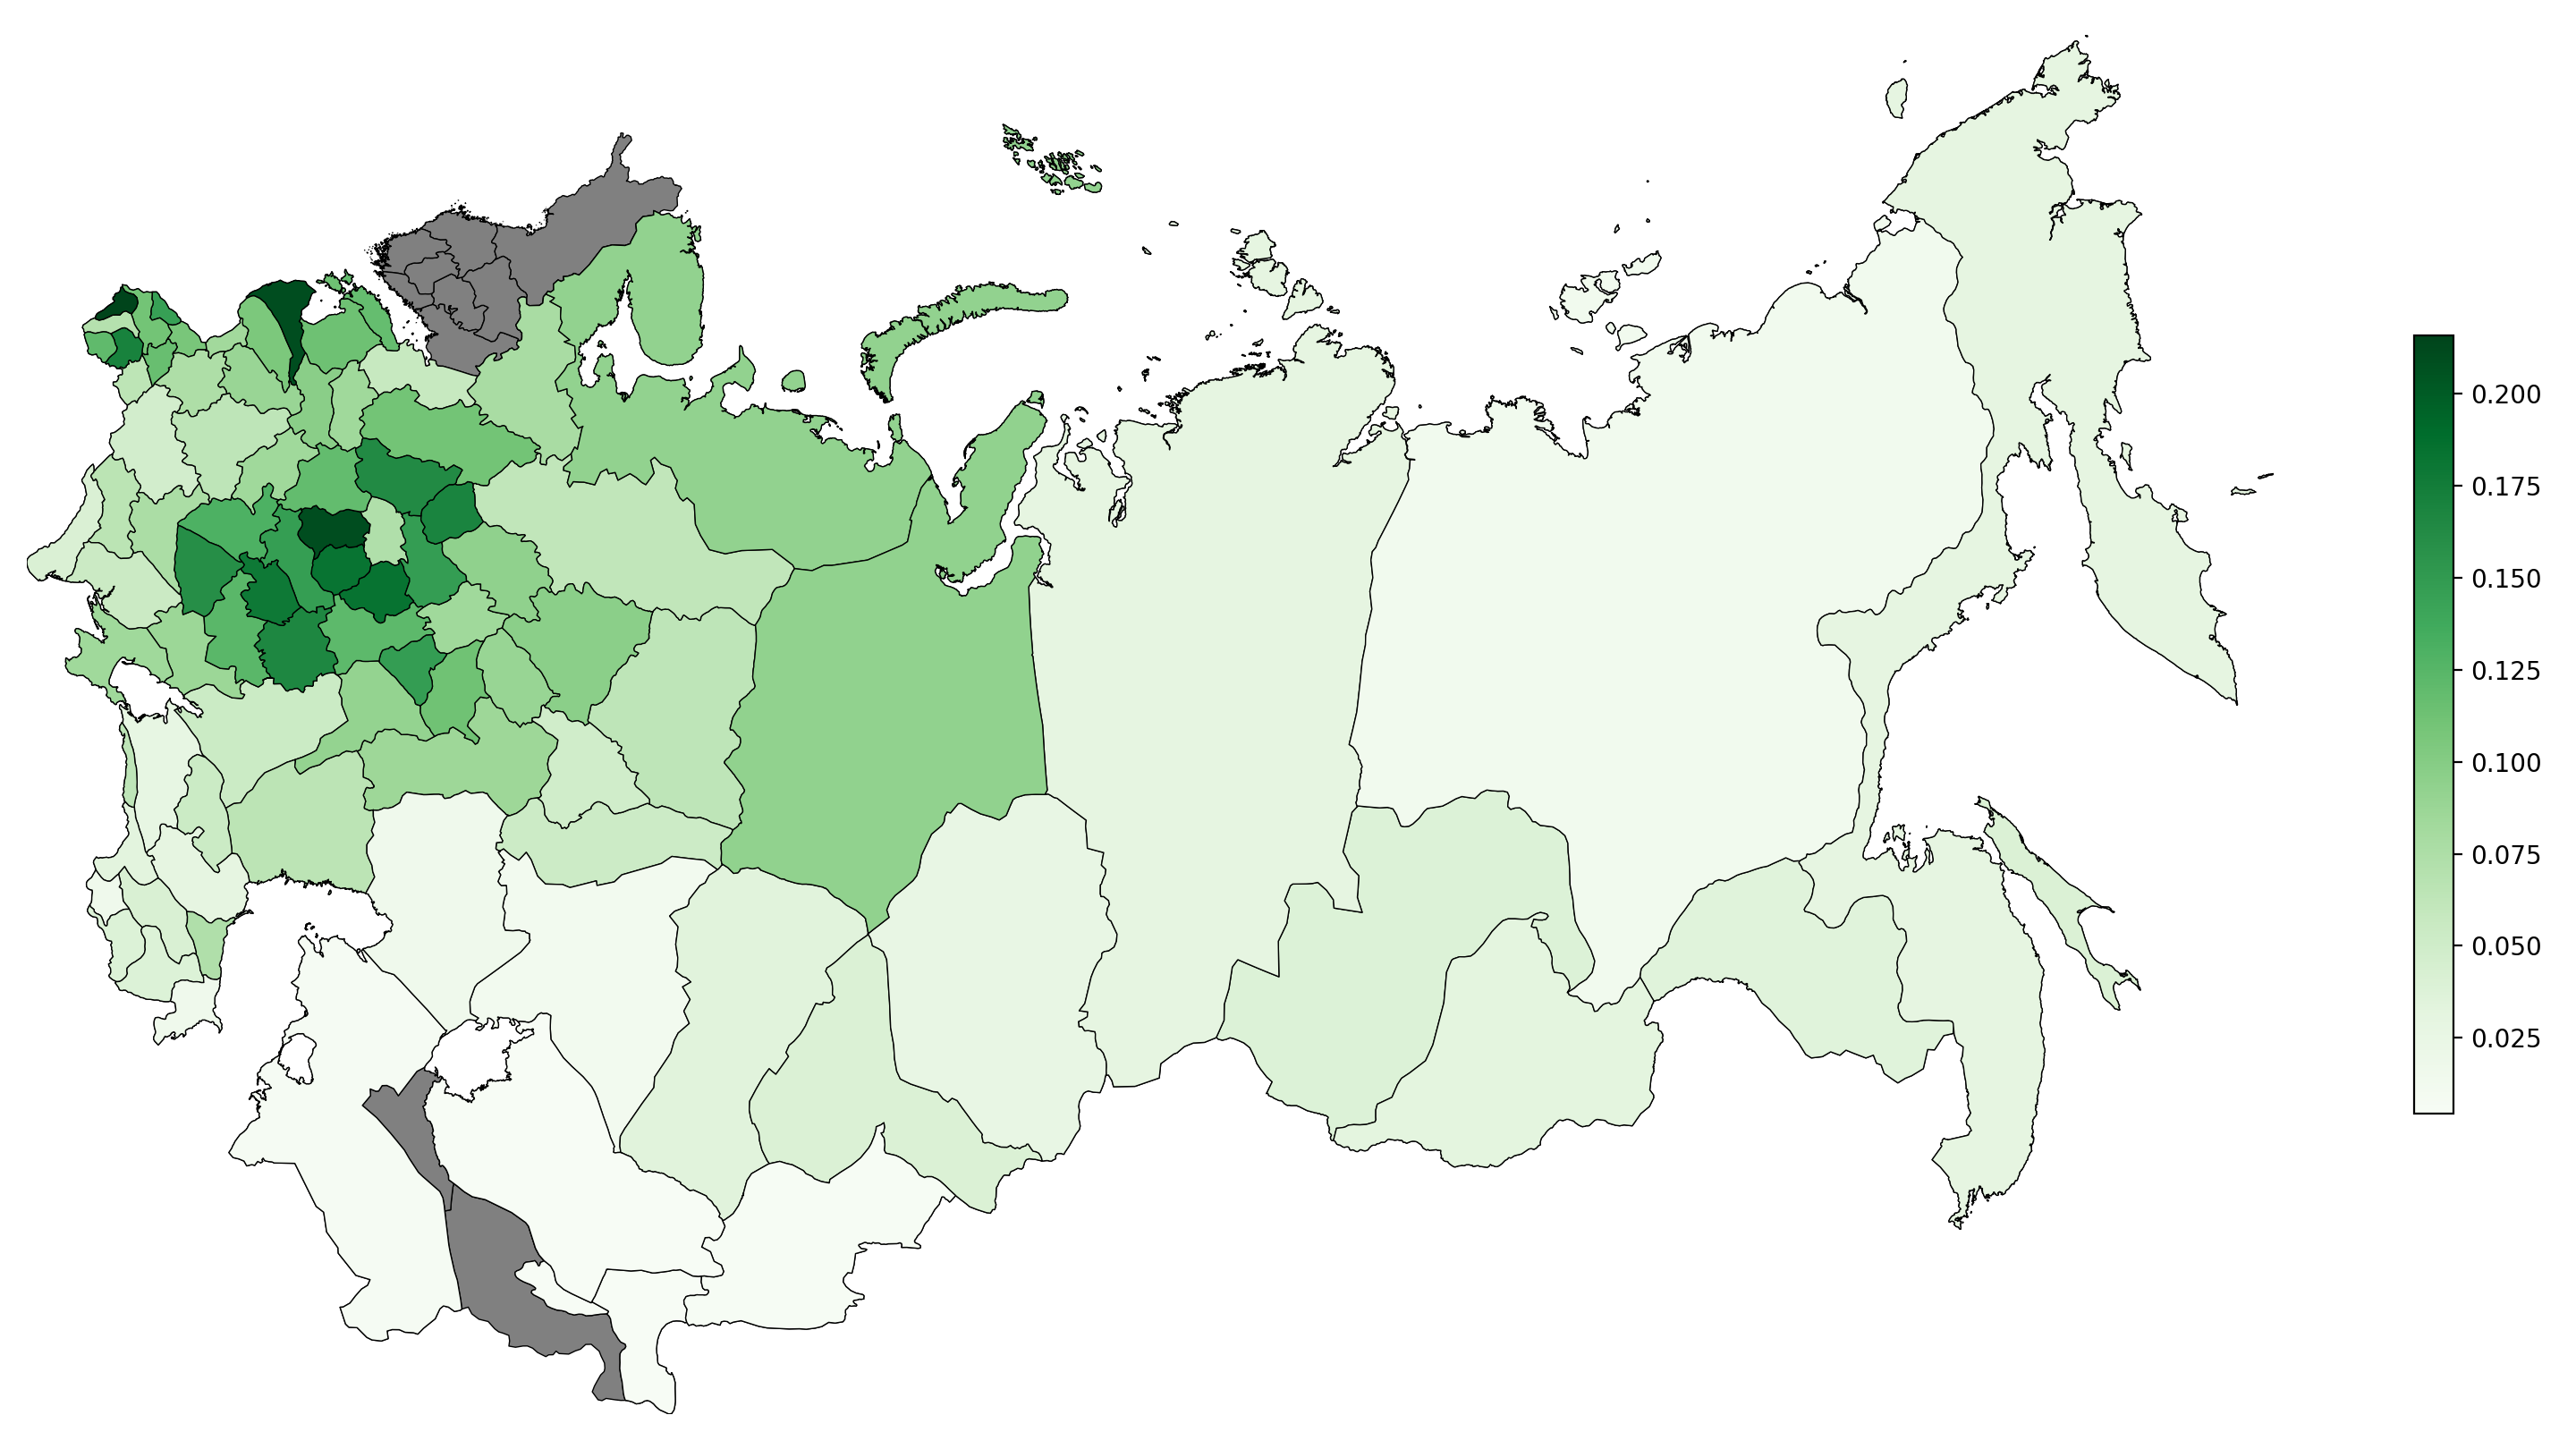
\includegraphics[height=0.85\textwidth]{mig_of_pop_from.png}
	\caption{Родившихся в регионе, но проживающих в других регионах, доля населения}
	\label{fig:from}
\end{figure}
	
\begin{figure}[h!]
	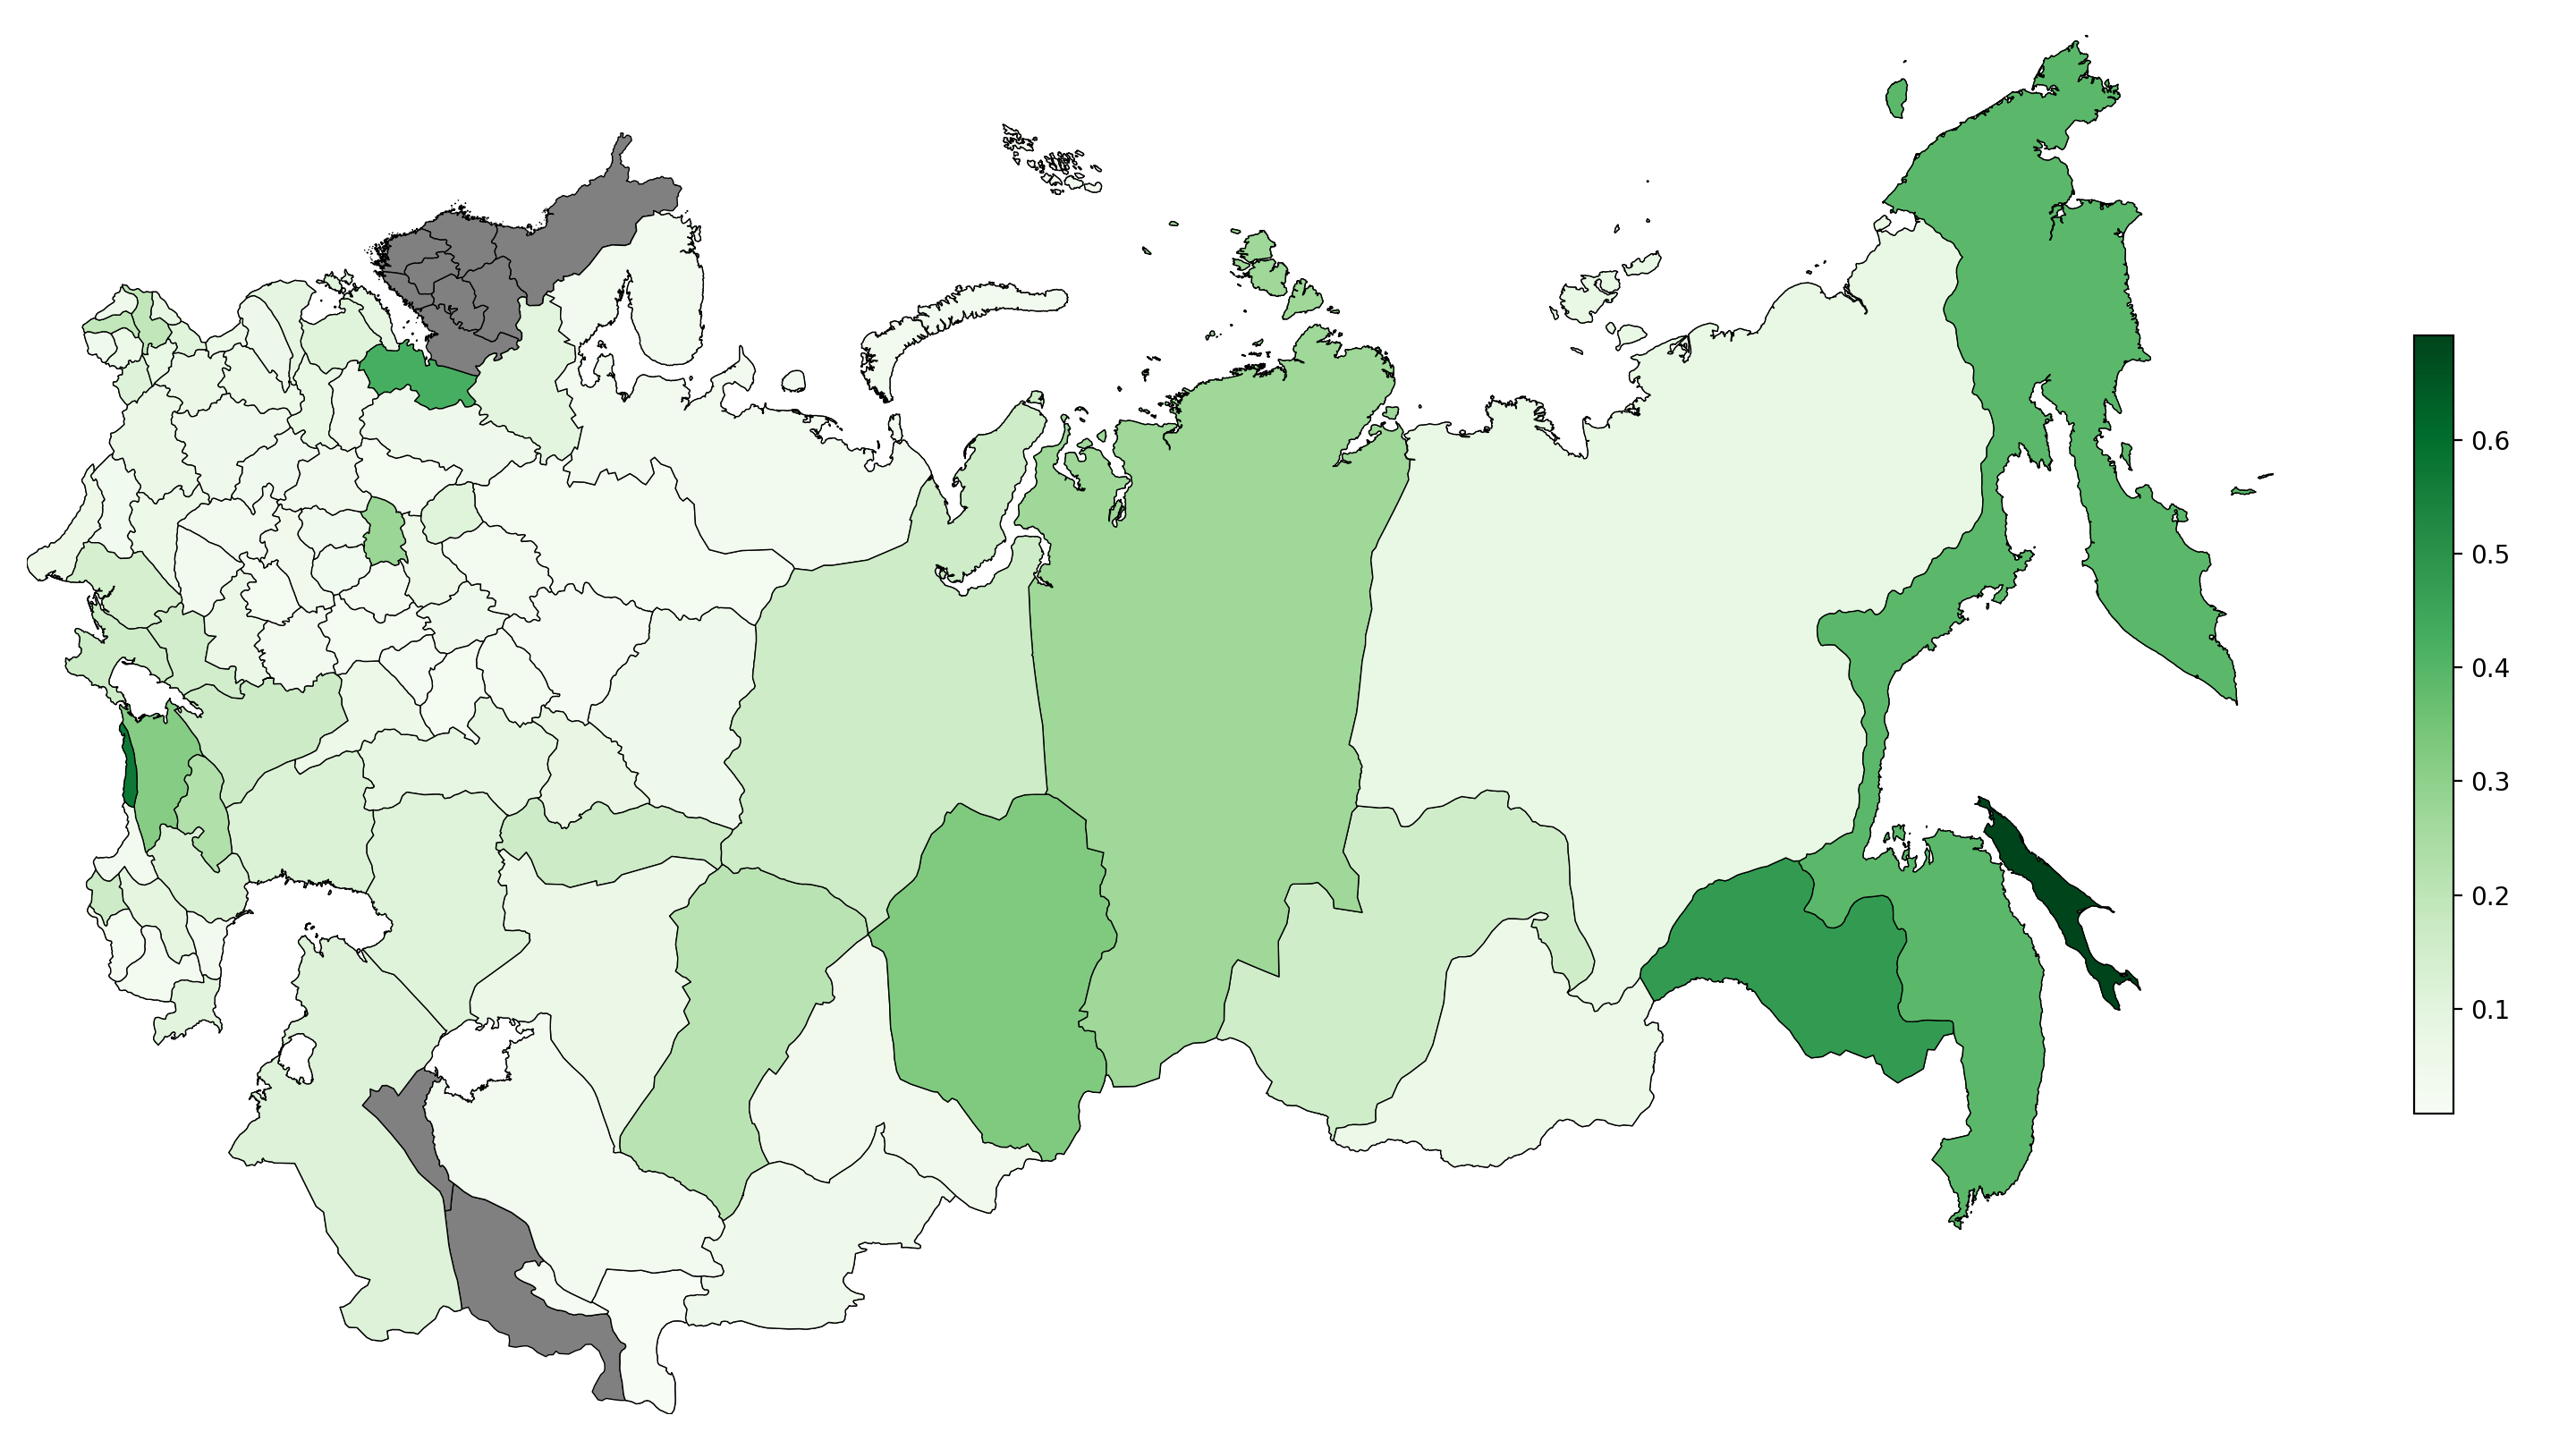
\includegraphics[height=0.85\textwidth]{mig_of_pop_to.png}
	\caption{Родившихся в других регионах, но проживающих в этом, доля населения}
	\label{fig:to}
\end{figure}

\end{landscape}

\end{document}
